\documentclass{article}
\usepackage[utf8]{inputenc}
\usepackage{hyperref}
\usepackage{color}

\author{Meng Lu, Joaquin Cavieres, Paula Moraga }
\date{September 2020}
\usepackage{amsmath}
\usepackage{natbib}
\setcitestyle{authoryear,open={(},close={)}} 
\usepackage{graphicx}
\usepackage{listings} 
\lstset{language=R,
    breaklines=true,
    basicstyle=\small\ttfamily,
    stringstyle=\color{DarkGreen},
    otherkeywords={0,1,2,3,4,5,6,7,8,9},
    morekeywords={TRUE,FALSE},
    deletekeywords={data,frame,length,as,character}
}
\usepackage{cleveref}
\usepackage{amsfonts}
 
\title{A comparison of geostatistical and non-spatial machine learning methods in $NO_2$ modelling: prediction accuracy, uncertainty quantification, and model interpretability }
\begin{document}




\maketitle
\begin{abstract} 
NO$_2$ is a traffic-related air pollutant that strongly associated with cardiovascular and lung diseases. Statistical prediction methods that captures relationships between NO$_2$ measurements and GIS or geospatial predictors, as well as the spatial structures of NO$_2$ have been developed to predict a continuous surface of NO$_2$. However, current studies comparing between various statistical models may not comprehensively evaluate different models. In this study, we dive into a systematic comparison process considering prediction accuracy, uncertainty quantification, and model interpretability across spatial algorithmic and non-spatial data models. Three cross-validation methods considering different levels and kind of spatial information are used to assess the prediction accuracy in different perspectives. Moreover, we evaluated stack learning methods with and without modeling spatial variations. We implemented our study using national ground station measurements of NO$_2$ in Germany and Netherlands of the year 2017, predicting NO$_2$ to 100 m resolution grid.   
%The probability distributions are calculated for latent Gaussian models and Random Forest models. The findings are extensible to boosting ensemble-tree methods. 
\end{abstract}
 
\textcolor{red}{In the abstract, what is the conclusion?}

\section{Introduction}
NO$_2$ is a highly local, traffic-related air pollutant and has been shown in clinics to associate with cardiovascular and lung diseases. High spatial resolution mapping NO$_2$ is required for providing scientific recommendations to police makers, as well as for studying the health impact and for risk assessment. Statistical methods for NO$_2$ mapping have attracted a lot of attentions with the burgeoning Machine Learning (ML) methods and availability of ground monitoring station networks, atmospheric satellite products, and geospatial predictors. Geospatial predictors are variables that are included as covariates in a statistical air polluton model. Commonly used geospatial predictors are for example air emission- (e.g. road networks) and dispersion-related (e.g. wind speed) variables, numerical modelling (e.g. with chemistry transport model) output, and atmospheric remote sensing measurements or products. An most recent (data available from Jan-2018) atmosphere sensing instrument, Tropomi (Tropospheric monitoring instrument, NSO and ESA, 2019) onboard of Sentinel 5p satellite, measures column density of a variety of gaseous air pollutants, in particular with an unprecedentedly high resolution for NO$_2$ (3.5 km x 5.5 km, across along track, since 06 August 2019). Statistical methods applied for spatial air pollution prediction can be broadly classified depending on whether the spatial dependency is explicitly modelled. If not modelled, we refer to the methods "non-spatial" and otherwise "spatial". 

Non-spatial methods are more dominant in air pollution mapping, particularly in high-resolution (100 m resolution or higher) mapping. Among them, LUR (land use regression) models which assumes linear relationships between NO$_2$ and geospatial predictors are the most studied \citep{briggs2000regression,hoek2008review}. Most recently, statistical learning (or machine learning) methods \citep{hastie2009elements}, including regularised linear regression (e.g. Lasso and Ridge regression \citep{James2013introduction}), kernel methods such as support vector machine \citep{svm1999least}, ensemble tree-based methods such as random forest (RF) \citep{breiman2001random} and boosting \citep{chen2016xgboost}, have been applied for feature selection or capturing non-linear response-covariate relationships \citep{luglobal,chen2019comparison}. In air pollution (not restricted to NO$_2$) mapping, several studies compared between statistical learning and conventional LUR methods  \citep{chen2019comparison,kerckhoffs2019performance,luglobal,REN2020105827,machinereview}.

Geostatistical models (e.g. Kriging) and Geographically weighted regression (GWR) are the most used spatial methods for air pollution prediction \citep{vicedo2013bayesian,li2014estimating,wang2021impacts,zou2016high} and these methods have been combined with dimension reduction \cite{zhai2018improved} and RF \citep{zhan2018satellite,liu2020integrate} to improve NO$_2$ prediction accuracy. A Bayesian geostatistical model is developed in \cite{BELOCONI2020105578} to predict NO$_2$ by integrating Tropomi satellite instrument measurements and chemical transport models. A GWR model fit multiple local regressions depending on the homogeneity in response-covariate relationships when a number of observations are involved and has been used to model spatial varying coefficients. A typical geostatistical model can be viewed as consisting two components: a mean function, commonly a linear model, capturing the response-covariate relationships and a covariance function modeling dependency of residuals from the mean \citep{stackinla}. In contrast to Geostatistical models and GWR, which identify the spatial structure based on the distance, the spatial autogressive model \citep{anselin2001spatial}, which models spatial effects based on neighbourhood connections (here ground station measurements), is studied in \cite{BERTAZZON20159}. Most of the spatial air pollution models predict at coarser resolutions, commonly 1 km or coarser \citep{young2016satellite,shaddick2018data,BELOCONI2020105578}.



%Machine learning methods commonly have a high predictive power but lower inference capability compared to a geostatistics methods. 


As spatial models are typically more complex compared to their non-spatial counter-parts, several studies compared spatial and non-spatial models to understand if the spatial effects could be simply modelled by including covariates in LUR models. \cite{young2016satellite} studied the use of universal Kriging (UK), OMI satellite instrument \citep{OMI} and LUR models for NO$_2$ prediction at 2.5 km resolution. \cite{young2016satellite} indicated that either using UK or adding OMI in the LUR model improves an LUR model but adding OMI in a UK model only trivially improves the performance. \cite{BERTAZZON20159} shows that the inclusion of the meteorological variables accounts spatial effects similarly as the use of spatial autoregressive models. However, even if the spatial dependency can be captured by involving certain covariates in a LUR model, we may still need geostatistical methods to understand the spatial structure present in the data. It can be viewed as consisting two components: a mean function capturing the relationship between independent variables and the response, and a covariance function modeling dependency of residuals from the mean \citep{stackinla}. Linear models have been used for the mean function; however, the relationships between NO$_2$ and predictors have been shown to be better modeled with non-linear machine learning methods \citep{luglobal}. Most recent studies attempt to replace the linear mean function with machine learning models. \cite{liu2020integrate} applies Gaussian process regression to the residuals from a random forest model, for the spatial prediction of PM$_2.5$. In disease mapping. \cite{stackinla} proposes to stack ML models to replace the mean function in a GP model.   

Few studies have compared between geostatistical and ML methods, possibly because the ML methods are still relatively new in air pollution mapping. It might be more interesting to compare between geostatistical methods and ML methods than geostatistical methods and LUR, because ML methods may be more flexibly in (implicitly) capturing spatial dependency by integrating covariates, when the number of observations is sufficient. Moreover, most comparison studies only compare the cross-validation accuracy of the prediction mean (e.g. using R-squared, mean absolute error, or root mean squared error), ignoring the prediction intervals. Also not discussed is the cause of the prediction errors, are they caused by missing co-variants, violation of the model assumptions (e.g. data distribution, non-linearity), or inconsistent distributions between training and validation sets? Also, different cross-validation strategies, e.g., how do we split the train-test sets, may lead to different model validation results. Current studies typically only use k-fold splitting \citep{kerckhoffs2019performance,larkin2017global,REN2020105827} or bootstrapping \citep{luglobal} to randomly splitting between train-test sets, which may be one-sided and does not provide an indication of accuracy in spatial blocks (but only at the point measurements). In this study, we focus on ensemble tree-based methods in the ML category and a hierarchical spatial model \citep{lindgren2011explicit} called latent Gaussian model in the geostatistics category. Additionally, we invest in stacked models in integrating ML and geostatistical models and develop a LUR model using Lasso for comparison.  
Ensemble trees are "nonparametric" models, deriving prediction intervals is therefore less straight-forward but can be achieved \citep{meinshausen2006quantile,wager2014confidence,stasinopoulos2007generalized,velthoen2021gradient}. One of the likely most widely recognisable method is Quantile Random Forest (QRF) \citep{meinshausen2006quantile}. QRF has been shown to estimate middle quantiles well but may fall short at the extremes due to the limited number of observations in the tail regions \citep{velthoen2021gradient}. \cite{velthoen2021gradient} proposed to use extreme quantile regression to estimate for data outside the range of observations. Another method is distributional regression forests (DF) \citep{schlosser2019distributional}, which embeds the GAMLSS \citep{stasinopoulos2007generalized} into RF.  

\cite{fouedjio2019exploring} compared prediction accuracy and uncertainty quantification between KED (Kriging with external drift) and QRF (quantile random forest) \citep{meinshausen2006quantile} by simulating data with various level of spatial dependency. It concluded that an optimal model choice depends on the level of spatial dependency and response-covariate relationships. However, it does not account for the fact that in practice, as an ensemble tree-based method can make use of a large of number of (possibly correlated) predictors without being constraint to a certain (e.g. linear) relationships, when the number of observations is sufficient, the spatial dependency may be explained by the covariates despite not being explicitly modelled. 


The objective is to compare geostatistics and non-spatial ensemble tree-based models for NO$_2$ mapping, in terms of their prediction accuracy, uncertainty quantification, and model interpretation and to understand effect of modeling spatial structures. More specifically, the following sub-objectives are reached:

\begin{enumerate}
    \item Optimising a hierarchical spatial model and ensemble tree-based models for NO$_2$ prediction.
    
    \item Developing a stacked ensemble model, i.e. a stack of various ML methods, which should have the highest predictive strength conditional to the data used, and a geostatistical model that use the stacked ensemble model to estimate its mean function \citep{stackinla}.
    \item Model comparison. 
\end{enumerate}

    %and their potential in providing information for model improvement (indicating missing co-variates).
 
%    \item Propose a framework for model comparison and spatial validation. 
    %and an optimal statistical model for high-resolution NO$_2$ mapping.
 
The gaussian latent model is implemented using INLA (Integrated Nested Laplace Approximation). XGBoost, Random Forest (RF) are chosen for the comparison with the GP regression and form the base learners in stacked learning. The ML methods are chosen for their dissimilarity: Lasso is a linear model without accounting for spatial dependency, which is modelled in a GP as spatial random effects \textcolor{red}{random effects?}. RF and XGBoost are non-linear and are not affected by dependent covariates. XGBoost is a highly scalable boosting method that builds tree models subsequently over the residuals of previous trees and has multiple routines to penalise model over-fittng \citep{xgboost}, which has been reported in various studies to obtain the highest prediction accuracy\cite{luglobal}. 

 
 
\section{Data}
NO$_2$ concentration measurements of 2017 from national ground stations of Germany and the Netherlands are used. The original hourly data is downloaded from EEA \citep{EEA}. Negative values are considered as missing. The data is aggregated to annual concentrations by taking the mean and omitting missing values. The spatial distribution of NO2 stations, histogram and Q-Q plot for normality are shown in \cref{fig:histqq}. %The urban type, "rural", "suburban", and "urban" are defined respectively by the population  < 300,  301 - 1500, and > 1500, within 1 km$^2$ \citep{urbantype}. 
A gamma distribution test is conducted using the method proposed in \cite{villasenor2015variance} and implemented in \cite{goft}.  The test result (p-value = 0.32) implies that the data distribution is not significantly different from gamma distribution. We also conducted a Shapiro test for normality, with the result implying the distribution of data being significant different from normal distribution (p-value= 8.605e-12).

\begin{figure}
    \centering
    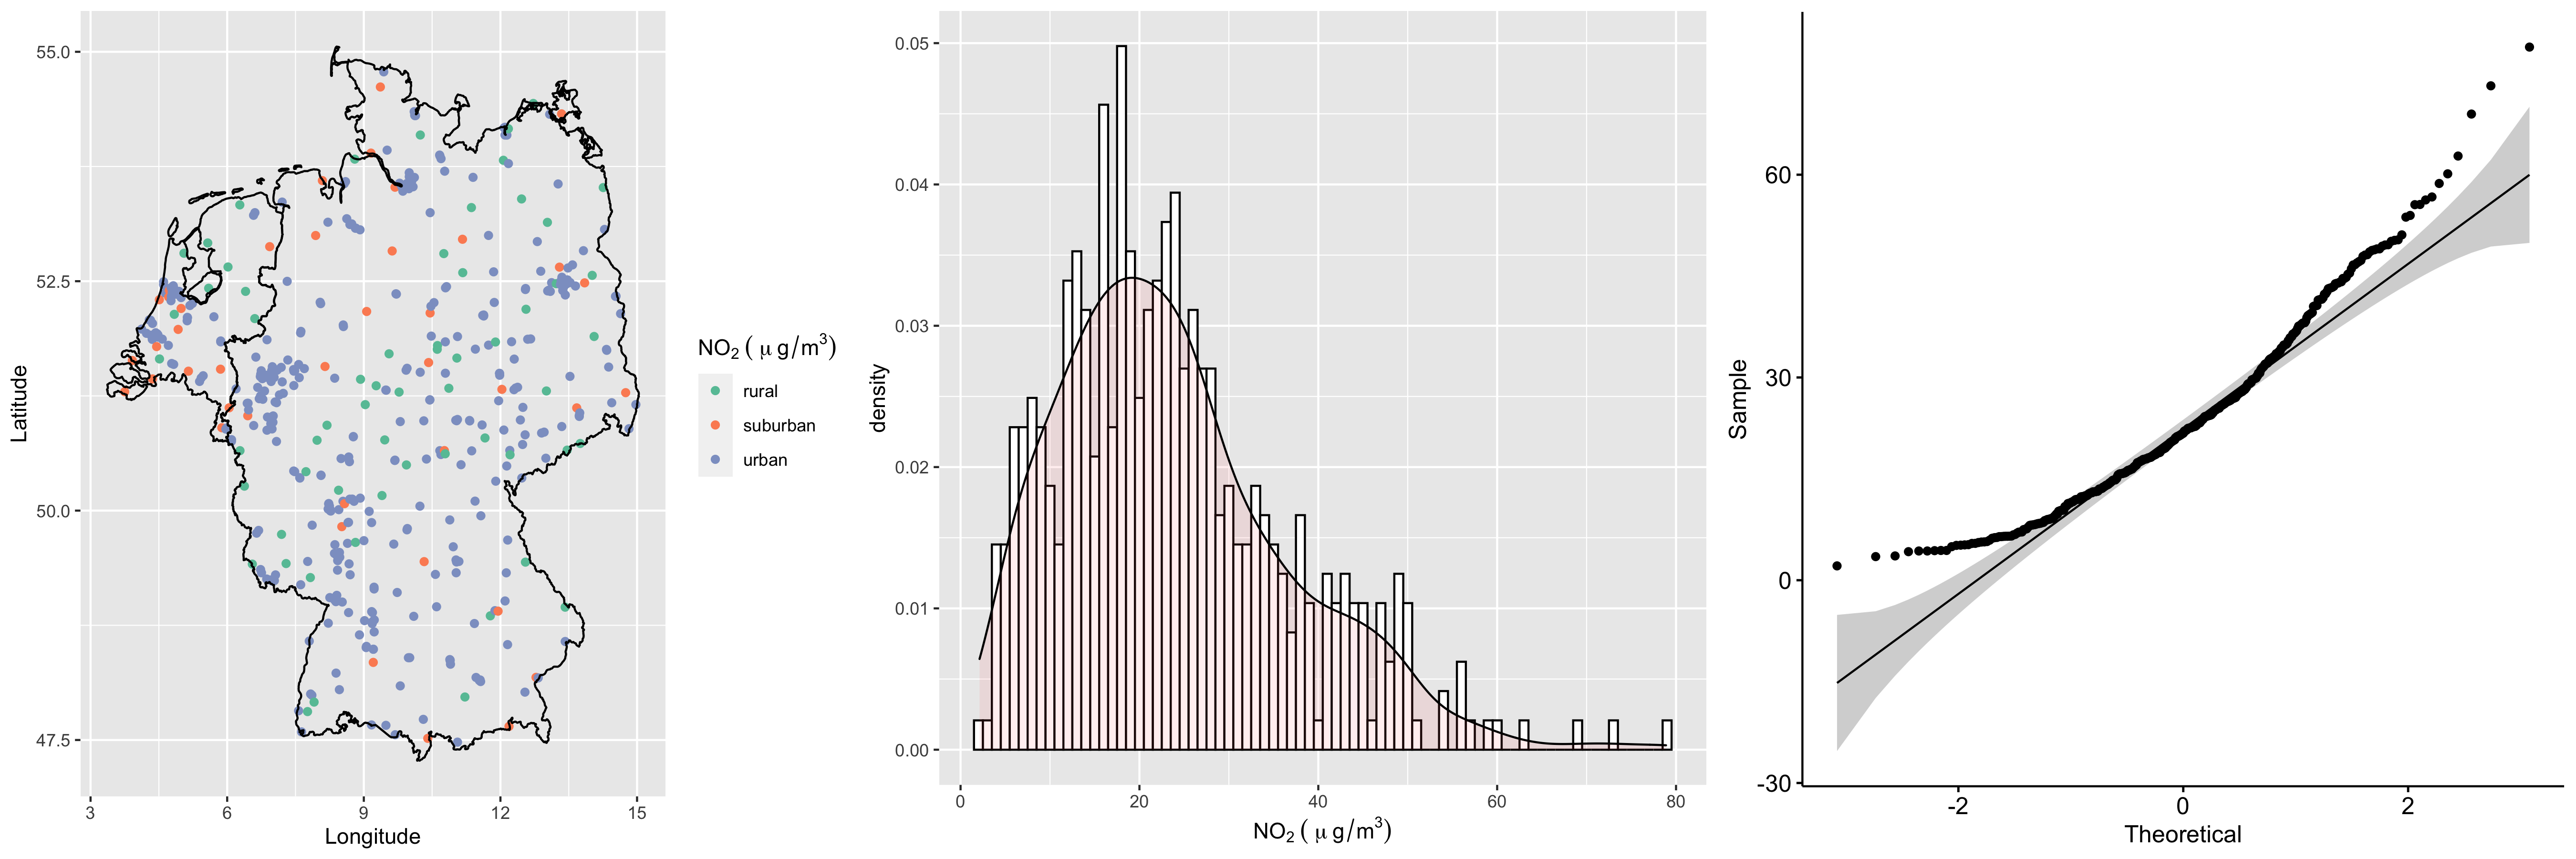
\includegraphics[scale=0.06]{fig/histqq_NO2.png}
    \caption{Spatial distribution of NO2 stations, histogram and Q-Q plot of the NO2 measurements.}
    \label{fig:histqq}
\end{figure}{}
The geospatial predictor grids (\cref{tab:prevar}) are calculated or re-sampled at 100 m resolution. They are either spatial attributes aggregated within a circular ring centred at each sensor or prediction location, called buffered predictors, or values of the spatial attribute at the observation or prediction location, called gridded variables. The buffered predictors include industry areas, roads, VIIRS (Visible Infrared Imaging Radiometer Suite) Nighttime Day/Night Band (DNB) radiance values \citep[nightlight,][]{nightlight} and population. Variables that are originally grids include wind speed and temperature \citep{dee2011era}, elevation \citep{amante2009etopo1}, monthly TROPOMI level 3 product of NO$_2$ column density  \citep{TROPOMIgee} from 2019 (due to the increased resolution compared to 2018). The buffered predictors of road and industry are calculated from OpenStreetMap  \citep{openstreetmap}. For detailed descriptions of the processing of the geospatial predictors please refer to \cite{luglobal}.   
 %OMI level 3 product of the 2017 annually aggregated NO$_2$ vertical column density, and the GEOS-CHEM \citep{bey2001global,GEOS-CHEM} annual NO$_2$ surface concentration product \citep{geddes2016long} of 2013. 

 
\begin{table}[h] 
\centering
\caption{Predictors used in this study. "\_mon" indicates months.  "\_buf" indicates the buffer radius in meters. The road length and industrial areas are calculated with buffer radii of 25 m, 50 m, 100 m, 300 m, 500 m, 800 m, 1000 m, 3000 m, 5000 m. The night lights digital numbers are calculated with buffer radii of 450 m, 900 m, 3150 m, 4950 m. The original resolution is provided for gridded (raster) variables and data types for vector variables.}

\label{tab:prevar}
{
\begin{tabular}{p{4cm}|l|l|l}
\hline
Predictor                                    & Variable name                & Unit         & Resolution/data type         \\ \hline
Monthly wind speed at 10 m altitude. &  Wind\_speed\_10m\_mon   & km/hr         &    10 km \\ \hline
Monthly temperature at 2 m altitude.  & temperature\_2m\_mon  &  Celsius        &    10 km \\ \hline
%OMI 2017 annual mean vertical column density. & OMI\_mean\_filt; OMI &  $mol /cm^2$ &    0.25 arc degrees \\ \hline
 
TROPOMI 2018 mean vertical column density.  & trop\_mean\_filt; Tropomi&  $mol /cm^2$ &   0.01 arc degrees  \\ \hline

%Remote sensing product generated of 2011 from \cite{geddes2016long} & RSp &$\mu g/ m^3$ & 10 km \\ \hline
Population in 5 km grid  & population\_5000 & count  & 5 km \\ \hline
Population in 3 km grid & population\_3000 & count  & 3 km \\ \hline
Population in 1 km grid  & population\_1000 & count  & 1 km\\ \hline
Nightlight  & nightlight\_bufnl & $W cm^{-2} sr^{-1}$  & 500 m\\ \hline
Total length of highway  & road\_1\_buf  & m &polygon, lineString              \\\hline
Total length of primary roads                   & road\_2\_buf          & m  &polygon, lineString            \\\hline
Total length of local roads     & road\_M345\_buf        & m  &polygon, lineString               \\\hline
Area of industry                                    & I\_1\_buf           & m$^2$ &polygon, lineString            \\\hline
 

\end{tabular}
}  
\end{table}

\section {Methods}

\subsection{Non-spatial methods}
Lasso is a linear regression algorithm with the L1 regularisation to shrink variable coefficients to zero, which enables "feature selection". In the cost function, the absolute value of coefficient is added to the original least squares as a penalty term. RF and XGBoost both use trees as base-learners and ensemble them to reduce variability of single trees \citep{friedman2001greedy}. RF firstly randomly draw a subset of features, and then choose features from the this subset to build the tree. RF \citep{breiman2001random} grows trees independently and then take the mean of the predictions of each tree. Additional to RF, we use Lasso as a post-processing of RF \citep[,][page 617]{hastie2017elements}. This method (called RFLA) firstly preserves all the trees instead of aggregatimng them (e.g. taking the mean of all the predictions) and then apply Lasso regression to all the trees for aggregation. This leads to a shrinkage of the tree space. We implemented this method using the QRF. 

QRF is a non-parametric method which keeps all the observations in the terminal node for estimating the conditional probability function. Specifically, it samples from all the response values in each terminal node and use the ratio between the number of samples that is taken from each terminal node and the number of total observations in the terminal node as weights to aggregate the samples. The weights of all the trees are summed and the summed weights computed for each observation are used to construct the empirical conditional cumulative distribution function \citep{meinshausen2006quantile}. DF \citep{schlosser2019distributional} firstly divide data into regions as homogeneous as possible with respect to a parametric distribution, thus capturing changes in location, scale and shapes. For each tree, maximum likelihood is used to fit distributions and recursively select and split co-variates according to the instability of the gradient of the likelihood at each observation along each co-variate. Then, the distributional trees are ensembled for DF.

XGBoost (XGB) is a variation of gradient boosting, which grows trees subsequently by fitting to current model residuals. XGB is scalable to multiple threads. It enables multiple penalisation paths to control model complexity to prevent model over-fitting, including regularisation (e.g. L1 regularisation) on tree width and terminal node values, as well as drop-out (dropping trees), sampling observations (take a subset of observations in each run), and early stopping (stop iterating when after a few rounds the loss does not decrease). The default objective function for regression assumes normal distribution of target variables (and the prediction is the mean of the distribution). This assumption is used in all the air pollution mapping studies. Here, we additionally fit a model with the objective function assuming the target variable follows a gamma distribution (called XGB-G) as the distribution of NO$_2$ measurements is closer to gamma than normal distribution.  

Different from the ensembling in RF or XGB, stacking ensemble (SE) refers to a class of algorithms that trains a second-level “meta-learner” to optimise the combination of a collection of prediction algorithms, which are known as base learners.  The learners are preferably to diverse to capture different relationships or patterns. In this study, Lasso, RF, and XGB are the base-learners. Cross-validated predicted values (commonly known as level-one data) are used to train the meta-learner. 

%\textcolor{red}{Here I would briefly describe each of the methods. Maybe just a 3-4 sentences. Merge the definition of the methods with section Modeling process}

\textcolor{red}{Regarding the Spatial modeling section about INLA, I would just define the geostatistical model for the observations. Then I would add only one or two paragraphs about how to fit the model using INLA and SPDE}

 
% INLA for model interpretatoin

%Among the ML methods, only the distribution prediction and interpretability from INLA and RF are compared, as INLA is representative to Gaussian process models and RF an ensemble tree model.
%The reason we choose random forest method to represent the XGB and Lasso is due to the good prediction accuracy obtained by RF+Lasso


%We refer Lasso and RF to excellent illustrations in classical machine books \citep{hastie2009elements,James2013introduction} and RF and XGBoost to the original papers \citep{breiman2001random,chen2016xgboost} and introduce INLA, RF+Lasso, and stacked modeling in the sections below.



\subsection{Spatial methods}

\subsubsection{Spatial random field}
A spatial random field is a stochastic spatial process generally defined by $\{X(\boldsymbol{s}): \boldsymbol{s} \in D \subset \mathcal{R}^{d}\}$, where $\boldsymbol{s}$ is the location in the space (e.g. latitude-longitude pairs) for the spatial process $X(\boldsymbol{s})$ and $D$ is the spatial domain. A spatial random field is a Gaussian random field if $\{X(\boldsymbol{s}_{1}),...., X(\boldsymbol{s}_{n})\} \sim \mathcal{N}_{n}(\boldsymbol{0}, \boldsymbol{\Sigma})$, where $N_{n}$ is a Normal multivariate distribution for the spatial process and is completely specified by it's mean $\mu = \mathbb{E}(X(\boldsymbol{s}))$, and the covariance function $C(\boldsymbol{s}_{1}, \boldsymbol{s}_{2}) = \text{Cov}(X(\boldsymbol{s}_{1}), X(\boldsymbol{s}_{2}))$. The Gaussian random field can be stationary and isotropic, where the covariance function depend only on the distance and not direction between points, that is $C(\boldsymbol{s}_{1}, \boldsymbol{s}_{2}) = \text{Cov}(\|\boldsymbol{s}_{1} - \boldsymbol{s}_{2}\|)$ and it's dependence is commonly modeled by a Matérn function (\cite{stein2012interpolation}\cite{yuan2011models}). Since incorporating the spatial dependence directly with a large number of observations using a Gaussian random field is computationally expensive, \cite{rue2005gaussian} proposed the approximation of a Gaussian random field by a Gaussian Markov random field for a more efficient computational process of estimation. The main property of the Gaussian Markov random field is that it uses a conditional dependency structure through the precision matrix $\boldsymbol{Q}$. INLA is used as an individual model and for stacked modeling with RF, XGB, and Lasso as covariates. 


\subsubsection{The SPDE (Stochastic partial differential equation) method}

To modeling data indexed in space, \cite{lindgren2011explicit} proposed a new methodology based mainly on the approximation of the Gaussian random field with the Matérn function using the Stochastic Partial Differential Equations (SPDE) as follow:

\begin{equation}\label{eqn:eq1}
(\kappa^{2} - \Delta)^{\alpha/2}(\tau(\boldsymbol{s}) x(\boldsymbol{s})) = \boldsymbol{\mathcal{W}(s)},
\end{equation}
 
where $\kappa$ is a scale parameter, $x(\boldsymbol{s})$ is a spatial random field, $\Delta$ is the Laplacian, $\alpha$ is the parameter that controls the smoothness of the realizations, $\tau$ controls the variance and $\boldsymbol{\mathcal{W}(s)}$  is a Gaussian spatial white noise process (\cite{lindgren2015bayesian}). For the above we can use a Gaussian Markov random field that approximates to a Gaussian random field without specifying an explicit covariance structure through the SPDE method. This approximation leads to a decrease in computational burden from $\mathcal{O}(n^{3})$ to $\mathcal{O}(n^{3/2})$. 


\subsubsection{Bayesian inference}

 The \texttt{R} package \texttt{INLA} facilitates the application of the Integrated Nested Laplace Approximation (INLA) method to performs direct numerical calculation of the posterior distribution for a Bayesian hierarchical model (\cite{rue2009approximate}\cite{martiNO$_2$009implementing}). If we use $\boldsymbol{x}$ as a latent Gaussian field (a Gaussian Markov random field), $\boldsymbol{\theta}$ a vector of (hyper)parameters and $\boldsymbol{y}$ a vector of observations, assuming independent observations given the vector of the spatial latent field ($\boldsymbol{x}$) and the hyperparameters ($\boldsymbol{\theta}$), the likelihood can be expressed as:

\begin{equation} \label{eqn:eq2}
p(\boldsymbol{y}\mid \boldsymbol{x},\boldsymbol{\theta}) =\prod_{i\in \mathcal{I}} p(y_i|\eta_i,\boldsymbol{\theta}),
\end{equation}

where $\eta_{i}$ is the linear predictor and $\mathcal{I}$ contains the indices for the observed values $\boldsymbol{y}$.  \\

The main idea is to approximate the posterior density for the posterior of the spatial latent field and the hyperparameters, hence, the marginal densities can be obtained:

\begin{equation} \label{eqn:eq3}
p(x_i \mid \boldsymbol{y}) = \int p(x_i \mid \boldsymbol{\theta},\boldsymbol{y})  p(\boldsymbol{\theta} \mid \boldsymbol{y}) d\boldsymbol{\theta},
\end{equation}
and
\begin{equation} \label{eqn:eq4}
p(\boldsymbol{\theta}_j|\boldsymbol{y}) = \int p(\boldsymbol{\theta} \mid \boldsymbol{y})  d\boldsymbol{\theta}_{-j}.
\end{equation}
respectively (\cite{lindgren2015bayesian}\cite{krainski2018advanced}). \\

\subsection{Model for data}

The general structure for a Bayesian hierarchical model in INLA is as follows:
\begin{align}
\boldsymbol{\theta} \hspace{2mm} \sim & \hspace{2mm} \pi(\boldsymbol{\theta}) \label{eqn:eq5}\\
\boldsymbol{x} \mid \boldsymbol{\theta} \hspace{2mm} \sim & \hspace{2mm} \mathcal{N}(\boldsymbol{0}, \boldsymbol{Q}(\boldsymbol{\theta})^{-1}) \label{eqn:eq6}\\
\eta_{i} \hspace{2mm} = & \hspace{2mm} \sum_{j}b_{ij}x_{j}\label{eqn:eq7}\\
\boldsymbol{y} \mid \boldsymbol{x}, \boldsymbol{\theta} \hspace{2mm} \sim & \hspace{2mm} \prod_{i \in \mathcal{I}}p(\boldsymbol{y} \mid \boldsymbol{\eta}, \boldsymbol{\theta}) \label{eqn:eq8},
\end{align}

where $\boldsymbol{\theta}$ is the vector of hyperparameters with $\text{log}(\tau) = \theta_{1}$ and $\text{log}(\kappa) = \theta_{2}$,  $\boldsymbol{x}$ is the spatial latent field, $\boldsymbol{\eta}$ is the linear predictor with covariates $b_{ij}$ and $\boldsymbol{y}$ is the vector of the response variable $f(\cdot \mid \boldsymbol{x}, \boldsymbol{\theta})$, commonly belonging from the exponential family of distributions. 
\vspace{0.2cm}

%We used "adaptive".
 
\subsection{Stacked Ensemble in a geostatistical model}
Extending from the non-spatial SE, a latent Gaussian model is used to stack the same base-learners but at the same time models the spatial random effects. Again, INLA is used to to implement and estimate the latent Gaussian model, with the same specification (i.e. mesh structure, likelihood, objective function, priors, optimisation process) as the INLA model described above. 

\section{Modeling process}
 
Models below are considered in this study. 
\begin{enumerate}
\item "INLA": a Gaussian latent model fit using INLA %assuming a Gaussian prior for NO$_2$ measurements \textcolor{red}{Model assumes priors for the different parameters. Do you mean assuming Gaussian distribution for NO$_2$ measurements?};
\item "LA": Lasso regression; 
\item "RF": Random forest; 
\item "XGB": XGBoost assuming a Gaussian objective function; 
\item "XGB-G": XGBoost assuming a Gamma objective function; 
\item "RFLA": RF in post-processing using Lasso \citep{hastie2009elements}, the QRF is implemented for RFLA; 
\item "SE": stacked learning of Lasso, RF, XGBoost models; 
\item "SE-INLA": stacked learning of Lasso, RF, XGBoost models using INLA;
\item "QRF": quantile regression forest \citep{meinshausen2006quantile};
\item "DF": distributional regression forest \citep{schlosser2019distributional}.
\end{enumerate}

The QRF and DF are not included in prediction accuracy comparison as the results are very similar to RF. Their prediction intervals are compared. 

\subsection{Hyperparameter setting for XGBoost and random forest}
\label{sec:hp}

To tune XGBoost, we used grid search to optimise hyperparameters in 5-fold cross-validation basing on the minimum RMSE (Root Mean Squared Error) and additionally manual adjustment of the hyperparameters to look at the prediction patterns. The search grid for the number of iterations (nrounds) was from 200 to 3000, with a step of 200; maximum tree depth (max-depth) from 3 to 6 with a step of 1, learning rate (eta) from 0.001 to 0.1 with a step of 0.05, the penalty term gamma \citep{xgboost}  from 1 to 5 with a step of 1, the subsample is set to 0.7, L1 norm penalisation (lambda) is set to 2 and L2 norm penalisation (alpha) is set to 0.  The optimal setting for RF is min.node.size equals 5 and mtry equals 12, the number of trees is set to 1000 for random forest, which is a safe choice as the high number of trees will not negatively affect model performance. The final setting for XGB is: nround = 3000, eta = 0.007, subsample = 0.7, max-depth = 6, gamma =5, lambda =2, alpha = 0. 

RF is not sensitive to hyperparameter tuning. We used the default setting of number of variables that are randomly drawn for each tree\citep{breiman2001random}, which is the integer part of the total number of variables divided by three. The number of trees is set to 1000. 


\subsection{Variable selection for INLA} 

For the INLA model, we used Lasso to reduce the number of variables. The Lasso is used in contrast to ensemble tree-based methods as they are both linear models. Variables are selected with the L1 norm penalty that returns an model with errors that are within one standard error of the minimum mean cross-validated error. Lasso is applied to 80\% data randomly sampled from all the observations and this process is repeated  20 times. Variables that are selected more than 90\% of the times (i.e. 18) will be considered as covariates in INLA. The frequency that the Lasso selected a certain variable is shown in \cref{lassoselect}. The INLA modeling process applies the same bootstrapped samples for training and validation.  In addition, AIC (step-wise) is applied to the entire dataset to suggest a model as a further reference. The variables selected by AIC is almost the same as Lasso selected variables, besides it does not choose road\_class\_3\_3000, which is highly correlated with  road\_class\_1\_5000. Therefore,  road\_class\_3\_3000 is not used as a covariate in INLA.  

  \begin{table}[!htbp] \centering 
  \caption{Frequencies (number of times) of variables selected by Lasso in 20 times bootstrapping and variables that are selected more than 90\% times (i.e. 18) are listed below. These variables are considered in INLA besides road\_class\_3\_3000.} 
  \label{lassoselect} 
\begin{tabular}{@{\extracolsep{5pt}} ccc} 
\\[-1.8ex]\hline 
\hline \\[-1.8ex] 
 & Variables & Frequency \\ 
\hline \\[-1.8ex] 
 1 & nightlight\_450 & $20$ \\ 
2 & population\_1000 & $20$ \\ 
3 & population\_3000 & $20$ \\ 
4 & road\_class\_1\_5000 & $20$ \\ 
5 & road\_class\_2\_100 & $20$ \\ 
6 & road\_class\_3\_300 & $20$ \\ 
7 & trop\_mean\_filt & $20$ \\ 
8 & road\_class\_3\_3000 & $19$ \\ 
9 & road\_class\_1\_100 & $18$ \\ 
%10 & road\_class\_3\_100 & $14$ \\ 
%11 & road\_class\_3\_5000 & $6$ \\ 
%12 & road\_class\_1\_300 & $5$ \\ 
%13 & road\_class\_1\_500 & $5$ \\ 
%14 & road\_class\_2\_1000 & $2$ \\ 
%15 & nightlight\_3150 & $1$ \\ 
%16 & road\_class\_2\_300 & $1$ \\ 
%17 & road\_class\_3\_1000 & $1$ \\ 
%18 & temperature\_2m\_7 & $1$ \\  
 
\hline \\[-1.8ex] 
\end{tabular} 
\end{table} 

\subsection{INLA model parameterisation}
Two INLA models are developed, one with Gaussian likelihood and the other with Gamma Likelihood. The mesh constructed is shown in supplementary  material (supfig. 1), with  size of the inner and outer extensions around the data locations (\textit{offsets}) 1/8 of the maximum distance among all the observations for both the inner and outer extensions. The maximum allowed triangle edge lengths in the region and in the extension (\textit{max.edge } ) are set to respectively 1/30 and 1/5 times maximum distance among all the observations. The Matern SPDE model is constructed with   $\alpha =2$. % and  with spatial scale parameter $\kappa$ a matrix of [0, 1, 0] and variance re-scaling parameter $\tau$ a matrix [0, 0, 1].

\section{Model evaluation}

\subsection{Cross validation}
We use MSE (root mean squared error), MAE (mean absolute value), IQR (interquartile range) and R$^2$ (R-squared) to compare model performance.   
RMSE is calculated as the square root of the differences between predictions and observations; MAE the absolute differences between predictions and observations; IQR the differences between the third and first quartiles of the prediction. R$^2$ indicates the explained variance and is calculated as $R^2 = 1- var(error) / var(y)$, where var(.) indicates variance, error indicates model residuals and y indicates observed response values. When different data is used in CV (e.g. separating between close and far-away from roads), we additionally calculated the RRMSE (relative RMSE), RMAE (relative MAE), RIQR (relative IQR) to account for the differences in the magnitudes of response values. The RRMSE and RMAE are calculated respectively by dividing the RMSE and MAE by the mean of observations. The RIQR was calculated by dividing the IQR by the median of observations.  

We designed three CV methods. 
\begin{enumerate}
\item Bootstrapped CV. 20-times random bootstrapped splitting of training and test sets \citep{luglobal}.  


 %   \item Probability sampling: higher probability is given to select observations that are isolated, to test how good the model is at predicting air pollution over the whole region. This is because with random sampling we would get more points in areas where observations are clustered and may not pick any observation in areas with few observations.   
\item Spatial-blocked CV. Dividing data into spatial blocks, each time use one block for test and other blocks for training. 
    
\item Customised CV. Splitting train-test based on values of certain covariates, in this study, three sub-areas are defined, 1) close to traffic and with high population ("tr-hp"), 2) close to traffic and with middle low population ("tr-lmp"), 3) far away from traffic ("far"). High population is defined as the variable population of 1000 m buffer that is in the last quartile. Low population is defined as the variable population of 1000 m buffer is below the median. Close to road is defined as (please refer to \cref{tab:prevar} for the definition of covariates): 
    \begin{lstlisting} 
    road_class_2_100 > 0 | 
    road_class_1_100 > 0 |
    road_class_3_100 > quantile(road_class_3_100, .75)) \end{lstlisting}
   
    Far away from road is defined as:
  \begin{lstlisting} 
    road_class_2_100 == 0 &
    road_class_1_100 == 0 & 
    road_class_3_100 < quantile(road\_class\_3\_100, .5)
    
    \end{lstlisting}
    where "{\tt \&}" indicates "and" and "{\tt |}" indicates "or". The second variable of the function "{\tt quantile(.)}" indicates the percentage quantile of the variables. 
   
    %\item Validation based on known attribute: we know the air quality station types (traffic, background, industrial) and human settlement types (urban or rural), this allows us to quantify prediction accuracy for each type of air quality stations and separating between urban and rural areas. 
\end{enumerate}
This yields 85, 65, and 177 samples in each category. This ensures a balanced number of samples between close to traffic and far-away from traffic. Each time, 30 samples (7\% of the entire dataset) are drawn from the corresponding category for CV. For example, each time, 30 samples are drawn from the 85 samples as the test set to obtain the prediction accuracy CV for the situation "tr-hp" and the rest is used for training.  

\subsection {Prediction intervals}
The CRPS (Continuous Ranked Probability Score) is an uncertain measure that assesses the similarities between two distributions.  We use it to indicates how the predicted distribution matches with the observed distribution. The CRPS implemented as an R package {\tt ScoringRules} \citep{jordan2017evaluating} is used. CRPS is calculated for the INLA and QRF (which represents ML-based methods). For the INLA model, The prediction intervals of INLA is calculated by simulating from the response Y $\sim N(\theta, sigma^2)$. The mean of CRPS for all the points within each test block is calculated in spatial-blocked CV.
 
%The coverage probability is calculated as the ratio between the number of  predictions within the upper and lower quantile and the total number of predictions. 
 

%inputs needed from Joaquine or Paula

 
\subsection{Model interpretation}
%Model interpretation is compared between INLA (linear model), RF and XGBoost, as they represent linear regression, bagging and boosting. 
We inspect fixed and spatial random effects modelled by INLA and compare the spatial random field with modelled prediction intervals and model residuals to understand the contribution of spatial random effects. Different from linear regression methods, which themselves are already the best models for interpretation, interpreting ensembling tree-based methods requires external models \citep{NIPS2017_8a20a862}. We use SHAP \citep[SHapley Additive exPlanations,][]{lundberg2018explainable,NIPS2017_8a20a862}, a unified method based on additive feature attribution, to estimate variable influence in RF and XGBoost models.   
%For a linear model like INLA, the best explanation model is the linear model itself but for ensembling methods it is harder to interpret the models \citep{NIPS2017_8a20a862}. We use SHAP \citep{NIPS2017_8a20a862} to interpret the ensemble tree models.


%\item XGboost
%Quantile regression is used to calculate the prediction quantiles of XGBoost, based on \cite{quantile} 

%\item Lasso


\section{Result and discussion}
\subsection{Accuracy assessment and uncertainty quantification}

\textbf{Non-spatial CV}
Both ensemble tree-based methods and INLA with Gaussian objective or likelihood obtain higher prediction accuracy than Lasso, indicating the necessity of using a more flexible model and modeling spatial random fields. Among individual methods, in terms of R$^2$ and RMSE, INLA with Gaussian likelihood obtained the highest prediction accuracy, followed by XGB-G and RFLA. RFLA greatly improves from original RF. Despite the distribution of response being closer to Gamma distribution compared to Gaussian distribution, using Gamma regression in XGB and specifying Gamma likelihood in INLA both decrease the prediction accuracy considerably. Compared to INLA, XGB obtained despite lower MAE  and IQR, lower RMSE and R$^2$, this indicates the XGB predict less well at more extreme ranges. 
 
 SE-INLA improves prediction accuracy compared to SE and INLA, obtained the lowest RMSE and the highest R$^2$ among all the models. This indicates the spatial structures could further improve prediction accuracy despite flexible relationships captured from ML models.
 
\begin{table}[!htbp] \centering 
  \caption{Prediction accuracy matrix for different models using 20 times bootstrapped cross-validation. LA: Lasso; RF: random forest, XGB: XGBoost using the default Gaussian loss; XGB-G: XGBoost using a gamma loss; RFLA: random forest with lasso for shrinkage aggregation of regression trees. INLA: Latent Gaussian model implemented using INLA assuming a Gaussian likelihood.} 
  \label{} 
\begin{tabular}{@{\extracolsep{5pt}} cccccccccc} 
\\[-1.8ex]\hline 
\hline \\[-1.8ex] 
         & LA  & RF   & XGB     & XGB-G & RFLA   & INLA  &INLA-G &SE& SE-INLA\\ 
\hline \\[-1.8ex] 
RMSE & $7.54$ & $7.45$ &$7.14$ & $8.91$ & $7.23$ & $7.06$ & 9.21 &7.18 & $6.83$\\ 
IQR & $8.47$ & $7.39$ & $6.54$ & $9.21$ & $7.27$ & $7.1$ & 7.4  &7.30& $6.8$\\ 
MAE & $5.69$ & $5.51$ & $5.05$ & $6.27$ & $5.28$ & $5.3$ & 6.2  &5.31& $5.0$\\ 
 
R$^2$ & $0.65$ & $0.65$ & $0.68$ & $0.51$ & $0.67$ & $0.69$ &  0.45& 0.69& $0.71$\\ 
\hline \\[-1.8ex] 
\end{tabular} 
\end{table} 

\textbf{Spatial-blocked CV}

Spatial-blocked CV provides information about prediction accuracy in spatial blocks. The R$^2$ map \cref{fig:r2} shows that the XGB, RF and INLA predict relatively well in most parts of Germany besides blocks at the boundaries. The R$^2$ for the block western the Netherlands is also relatively low with all the three methods and especially for XGB (R$^2$: 0.2). RF obtains the best result for the block of western the Netherlands (R$^2$: 0.5). The INLA model outperforms RF and XGB in the blocks at south-east and north. The R$^2$ between blocks are the most heterogeneous with XGB, which consists with the bootstrapped CV result that it falls short at predicting extremes.  

The spatial-blocked CRPS\cref{fig:crps} is computed for QRF and INLA (the DF is not shown as it will be shown that the QRF and DF performed similarly \cref{sec:predinterval}). The INLA predicted prediction distribution deviate considerably from observed distribution for the block of western the Netherlands, as reflected by the high value of mean CRPS. This consists with the relatively low R$^2$ observed for the same block. However, some blocks with relatively high R$^2$ (in the north and south) have high CRPS. This indicates that the prediction mean is well-predicted but not the prediction interval, which is likely too narrow. 

\begin{figure}
    \centering
    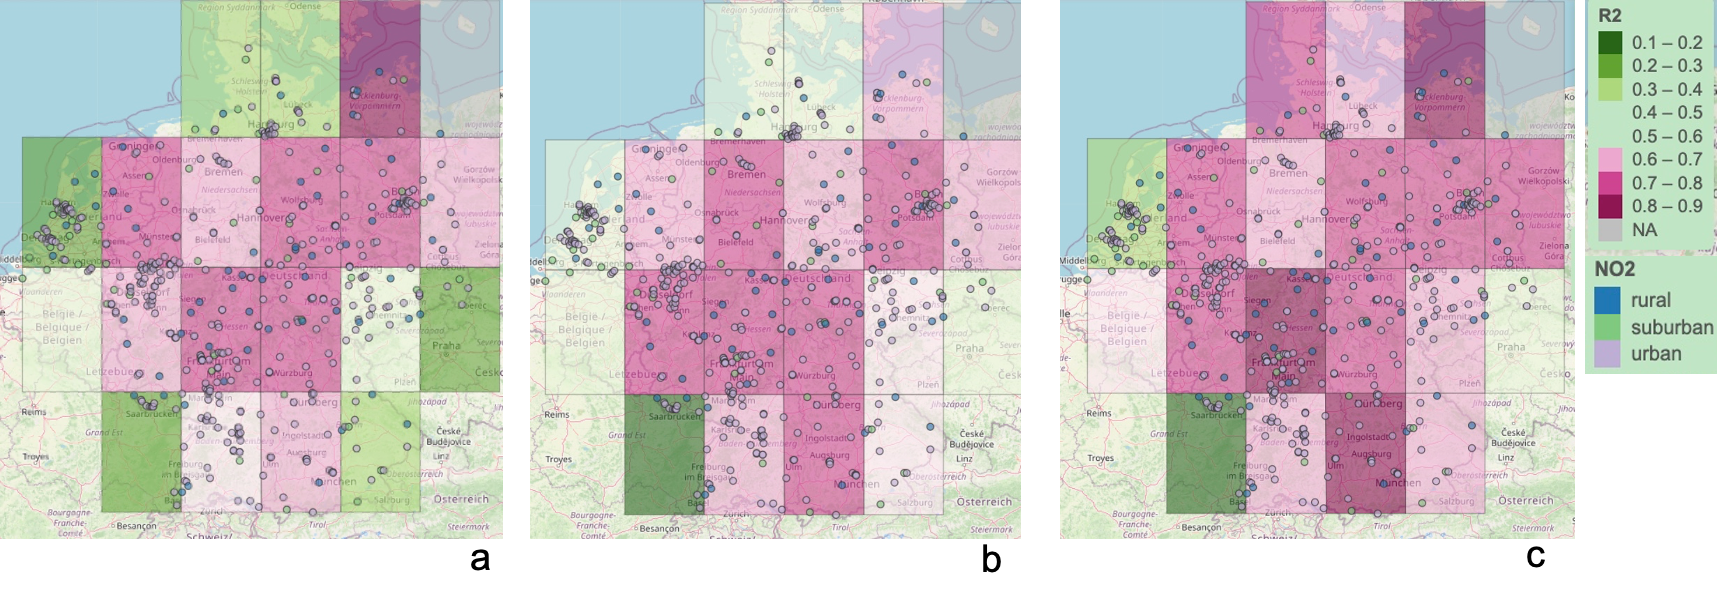
\includegraphics[scale=0.4]{fig/r2spcv.png}
    \caption{The R-squared of each block, using the rest of the blocks for training. The models are a) XGB, b) QRF, c) INLA. 
}
    \label{fig:crps}
\end{figure}

\begin{figure}
    \centering
    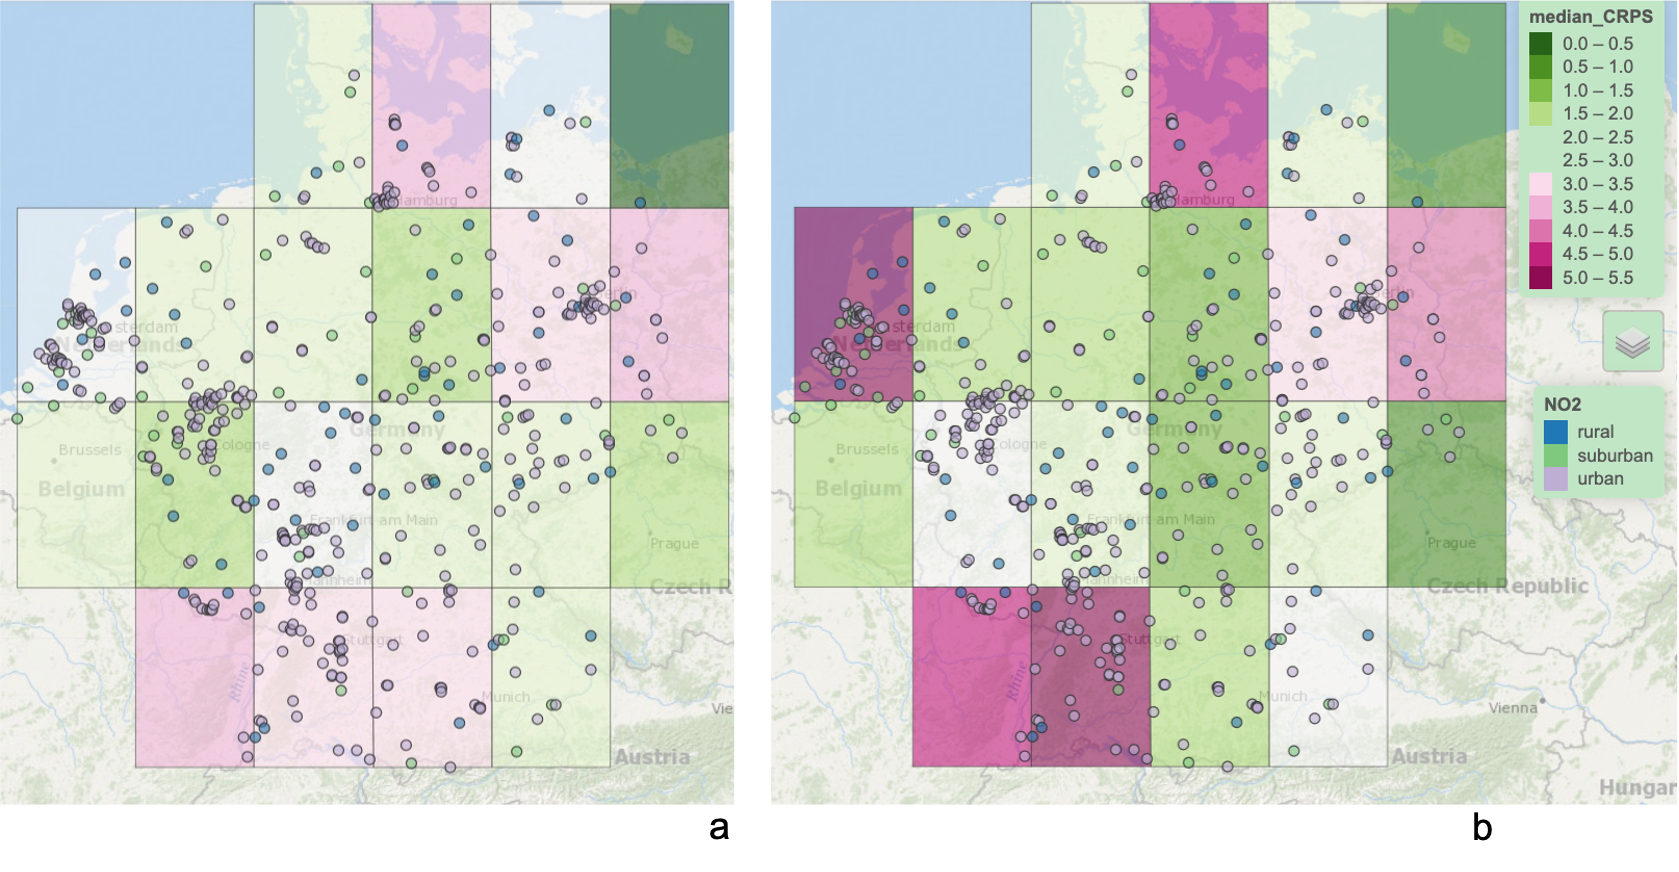
\includegraphics[scale=0.3]{fig/crps_RF_INLA.png}
    \caption{The CRPS (Continuous Ranked Probability Score) of each block, using the rest of the blocks for training. a) RF, b) INLA. 
}
    \label{fig:r2}
\end{figure}


\textbf{Customised CV}
There is a distinctive difference between model performance in areas close to traffic (i.e. \textit{tr-hp} and \textit{tr-lmp}) and far away from traffic (i.e. \textit{far}). The INLA model outperformed other non-spatial methods in both \textit{tr-hp} and \textbf{tr-lmp}, especially for the latter while the XGB model outperformed the INLA model (and all the other models) in \textit{far}. This indicates the importance of modeling spatial dependency in areas close to traffic and possibly non-linear relationships far-away from roads. All the ensemble tree-based methods obtained much worse results compared to linear regression methods in \textit{tr-lmp}. A linear regression model typically outperform ensemble tree-based methods when there are relatively few observations for a flexible relationship to be justified. As the number of observations that are close to traffic and far-away from traffic is balanced, the results indicates that the population density alters relationships between NO2 and road density (i.e. the relationships between NO2 and road density is different with different population density) in areas close to traffic. 

\begin{table}[!htbp] \centering 
  \caption{Results with customised CV. tr-hp: close to traffic and high population, tr-lmp: close to traffic and middle and low population, far: far away from traffic. RRMSE (relative RMSE), rMAE (relative MAE), rIQR (relative IQR).} 
  \label{customisedCV} 
\begin{tabular}{@{\extracolsep{5pt}} cccccccc} 
\\[-1.8ex]\hline 
\hline \\[-1.8ex] 
 & RMSE & RRMSE & IQR & rIQR & MAE & rMAE & R$^2$ \\ 
\hline \\[-1.8ex] 
LA\_tr-hp & $12.4$ & $0.3$ & $17.3$ & $0.4$ & $10.2$ & $0.3$ & $0.11$  \\ 
RF\_tr-hp & $11.9$ & $0.3$ & $17.8$ & $0.5$ & $9.8$ & $0.3$ & $0.18$   \\ 
XGB\_tr-hp & $11.6$ & $0.3$ & $15.3$ & $0.4$ & $9.3$ & $0.2$ & $0.21$ 
\\
INLA\_tr-hp & $11.3$ & $0.3$ & $16.6$ & $0.4$ & $9.5$ & $0.3$ & $0.26$
\\ 
\hline
LA\_tr-lmp & $7.5$ & $0.3$ & $10.4$ & $0.5$ & $6.1$ & $0.3$ & $0.21$ 
\\ 
RF\_tr-lmp & $8.2$ & $0.4$ & $10.9$ & $0.5$ & $6.4$ & $0.3$ & $0.05$  \\ 
XGB\_tr-lmp & $8.2$ & $0.4$ & $10.5$ & $0.5$ & $6.4$ & $0.3$ & $0.04$   \\ 
INLA\_tr-lmp & $6.7$ & $0.3$ & $8.7$ & $0.4$ & $5.3$ & $0.2$ & $0.36$ \\ 

\hline
LA\_far & $5.0$ & $0.4$ & $4.9$ & $0.4$ & $4.2$ & $0.3$ & $0.47$  \\ 
RF\_far & $4.9$ & $0.3$ & $4.0$ & $0.3$ & $3.6$ & $0.3$ & $0.47$  \\ 
XGB\_far & $3.4$ & $0.2$ & $3.6$ & $0.3$ & $2.5$ & $0.2$ & $0.74$   \\ 
INLA\_far & $4.0$ & $0.3$ & $4.3$ & $0.3$ & $3.2$ & $0.2$ & $0.65$

\\
\hline 
\\[-1.8ex] 
\end{tabular} 
\end{table} 

\subsection{Prediction interval}
\label{sec:predinterval}
\begin{figure}
\centering
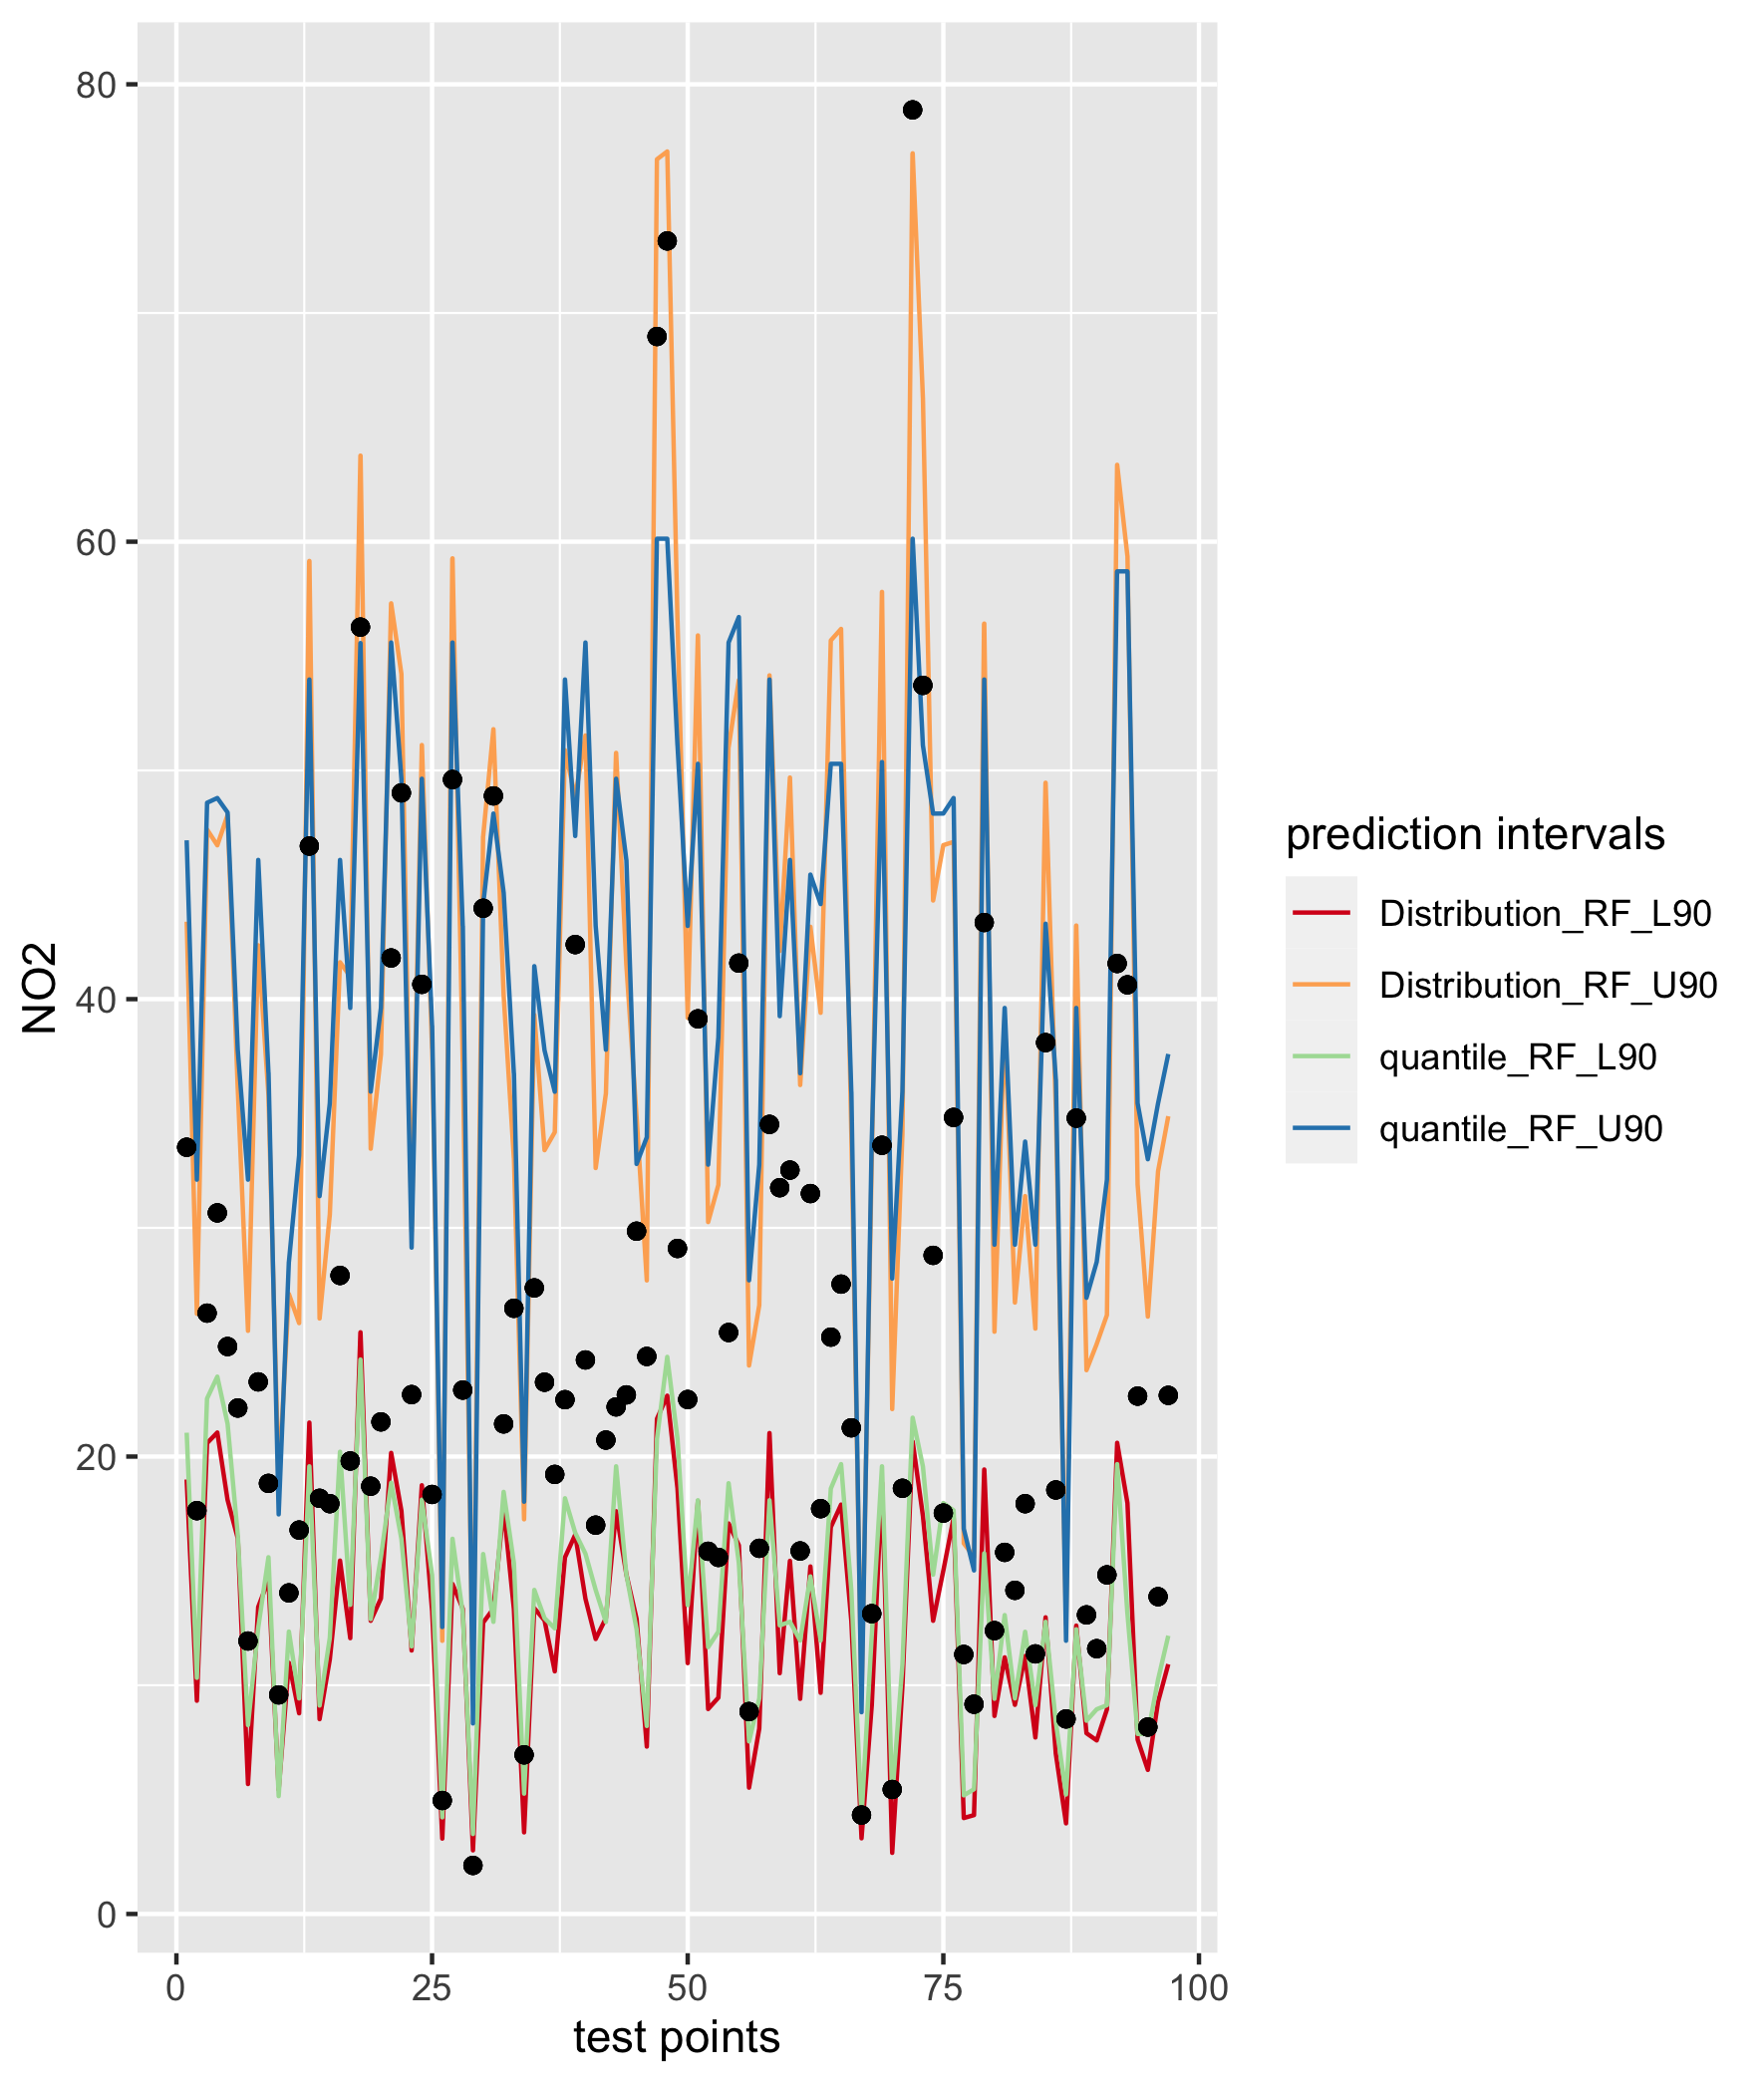
\includegraphics[scale = 0.2]{fig/dist_vs_qrf.png}
\caption{The 90\% prediction interval predicted by distributional forest and quantile regression trees. The black dots indicate observations in the test dataset.}
\label{distvsquant}
\end{figure}

Both the distributional forest and quantile regression trees reach the coverage probability higher than 0.9, but the distributional forest predict a more realistic prediction quantile, notably, it covers four observations that are not covered by the prediction quantile predicted by the quantile regression forest. 

\subsection{Model Interpretation} 
%For a linear model the best explanation model is the linear model itself but it is harder to interpret ensembling models \citep{NIPS2017_8a20a862}, which we used SHAP \citep{NIPS2017_8a20a862}.

SHAP values are calculated for RF and XGB methods using all the data. The variables are ranked by their variable importance, which is calculated as the sum of SHAP magnitudes over all the samples. It can be observed from \cref{rfshap} and \cref{xgbshap} that the variable rankings are similar and the number of points that have positive or negative impact are similar. Both methods ranked road\_class\_2\_100 at the top. The SHAP values also indicate a realistic pattern of the sample influence. For example, low  road\_class\_2\_100 values have low SHAP values and high road\_class\_2\_100 values have high SHAP values, this matches with the explanation that areas with higher primary road density generally have higher NO2.

% do they give the same interpretation?
\begin{figure}
\centering
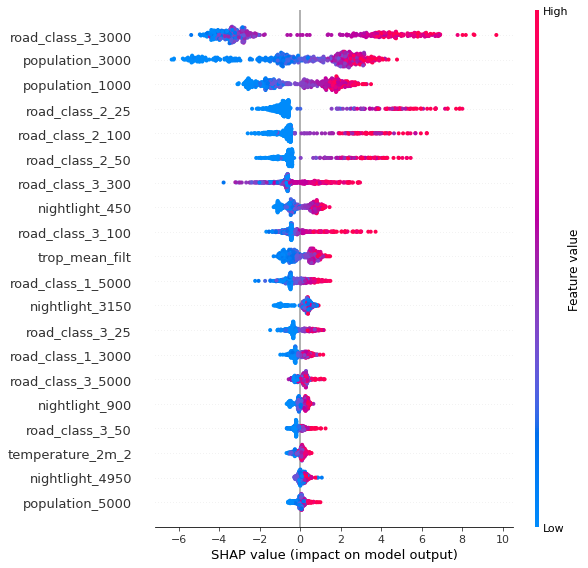
\includegraphics[scale = 0.5]{fig/rfshap.png}
\caption{Variable impact calculated by SHAP, the RF model. The horizontal location shows whether the effect of that value is associated with a higher or lower prediction. The ranking is based on the sum of SHAP magnitudes over all the samples.}
\label{rfshap}
\end{figure}

\begin{figure}
\centering
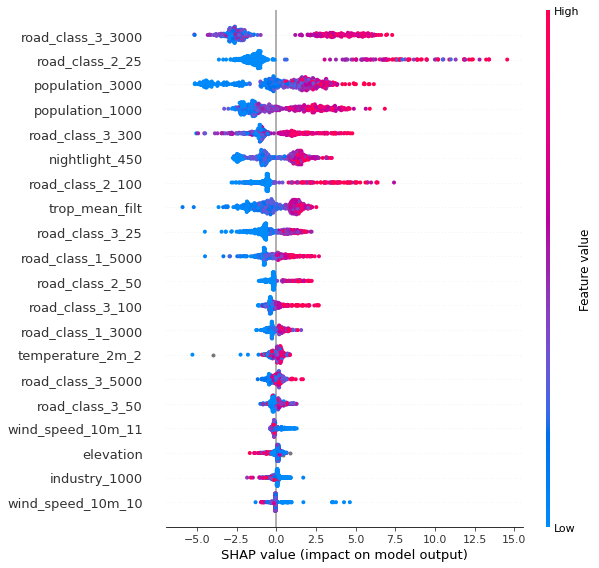
\includegraphics[scale = 0.5]{fig/xgbshap.png}
\caption{Variable impact calculated by SHAP, the XGBoost model. The horizontal location shows whether the effect of that value is associated with a higher or lower prediction. The ranking is based on the sum of SHAP magnitudes over all the samples.}
\label{xgbshap}
\end{figure}

The spatial random field estimated by the INLA model is shown in \cref{randomfield}. Patches of high values are shown 
\begin{figure}
\centering
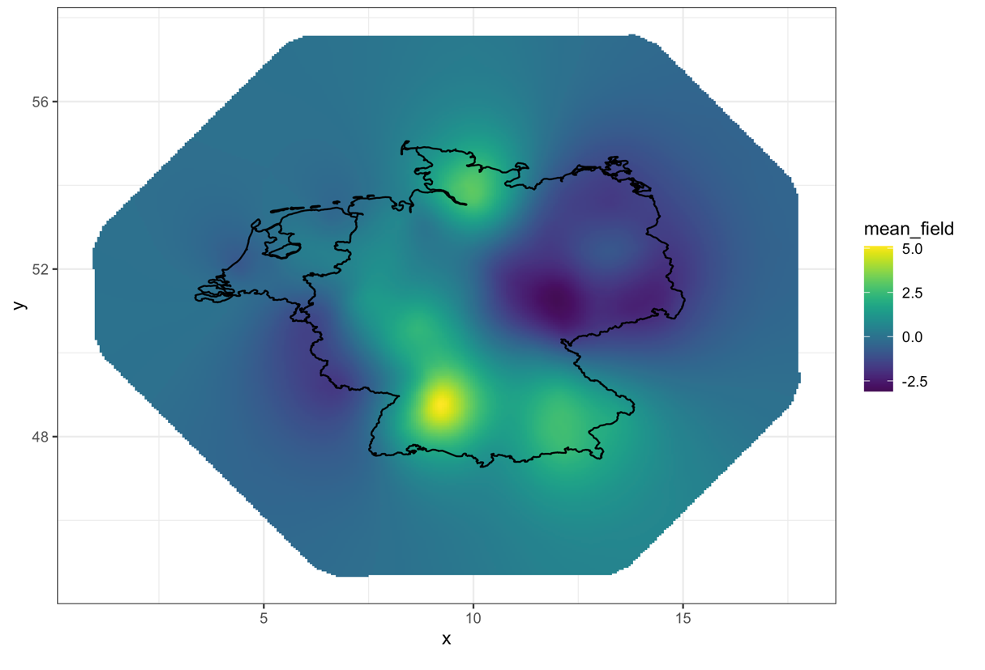
\includegraphics[scale = 0.5]{fig/mean_randomfield.png}
\caption{Mean random field fit by the INLA model.}
\label{randomfield}
\end{figure}


\begin{figure}
\centering
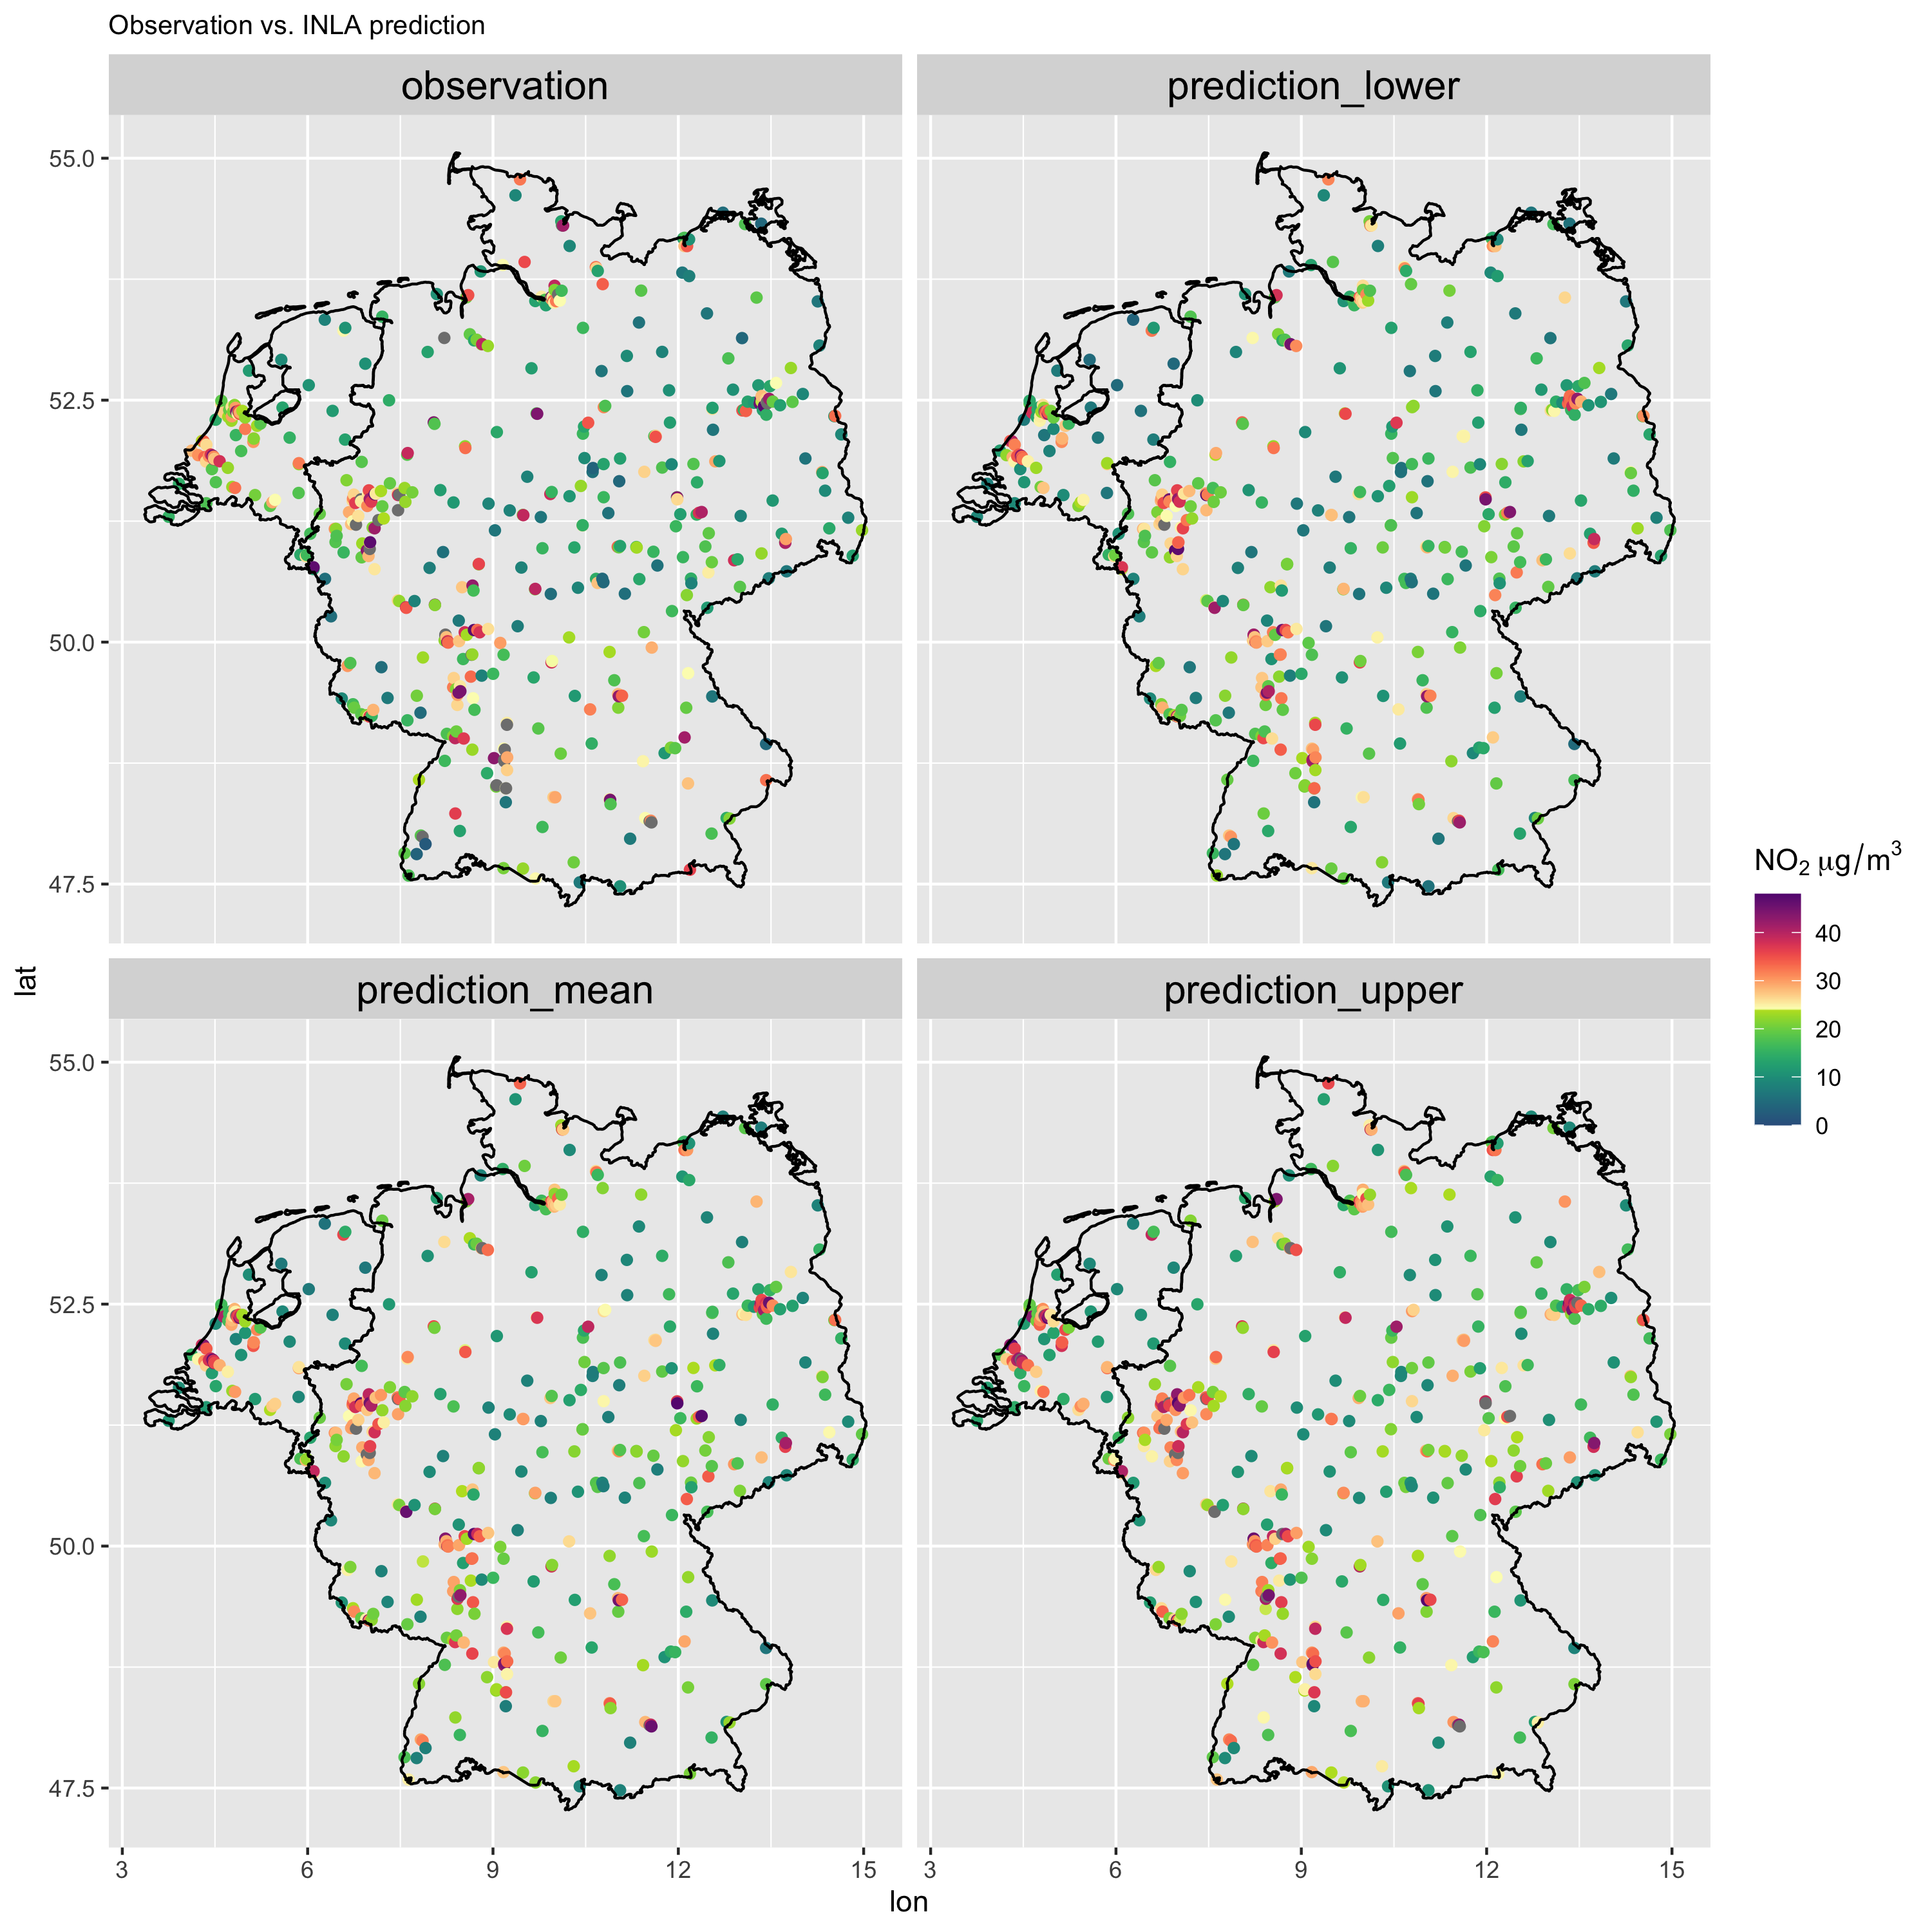
\includegraphics[scale = 0.05]{fig/pred_11var.png}
\caption{INLA predicted NO2 at the ground stations and the observed NO2. }
\label{INLApred}
\end{figure}

\begin{figure}
\centering
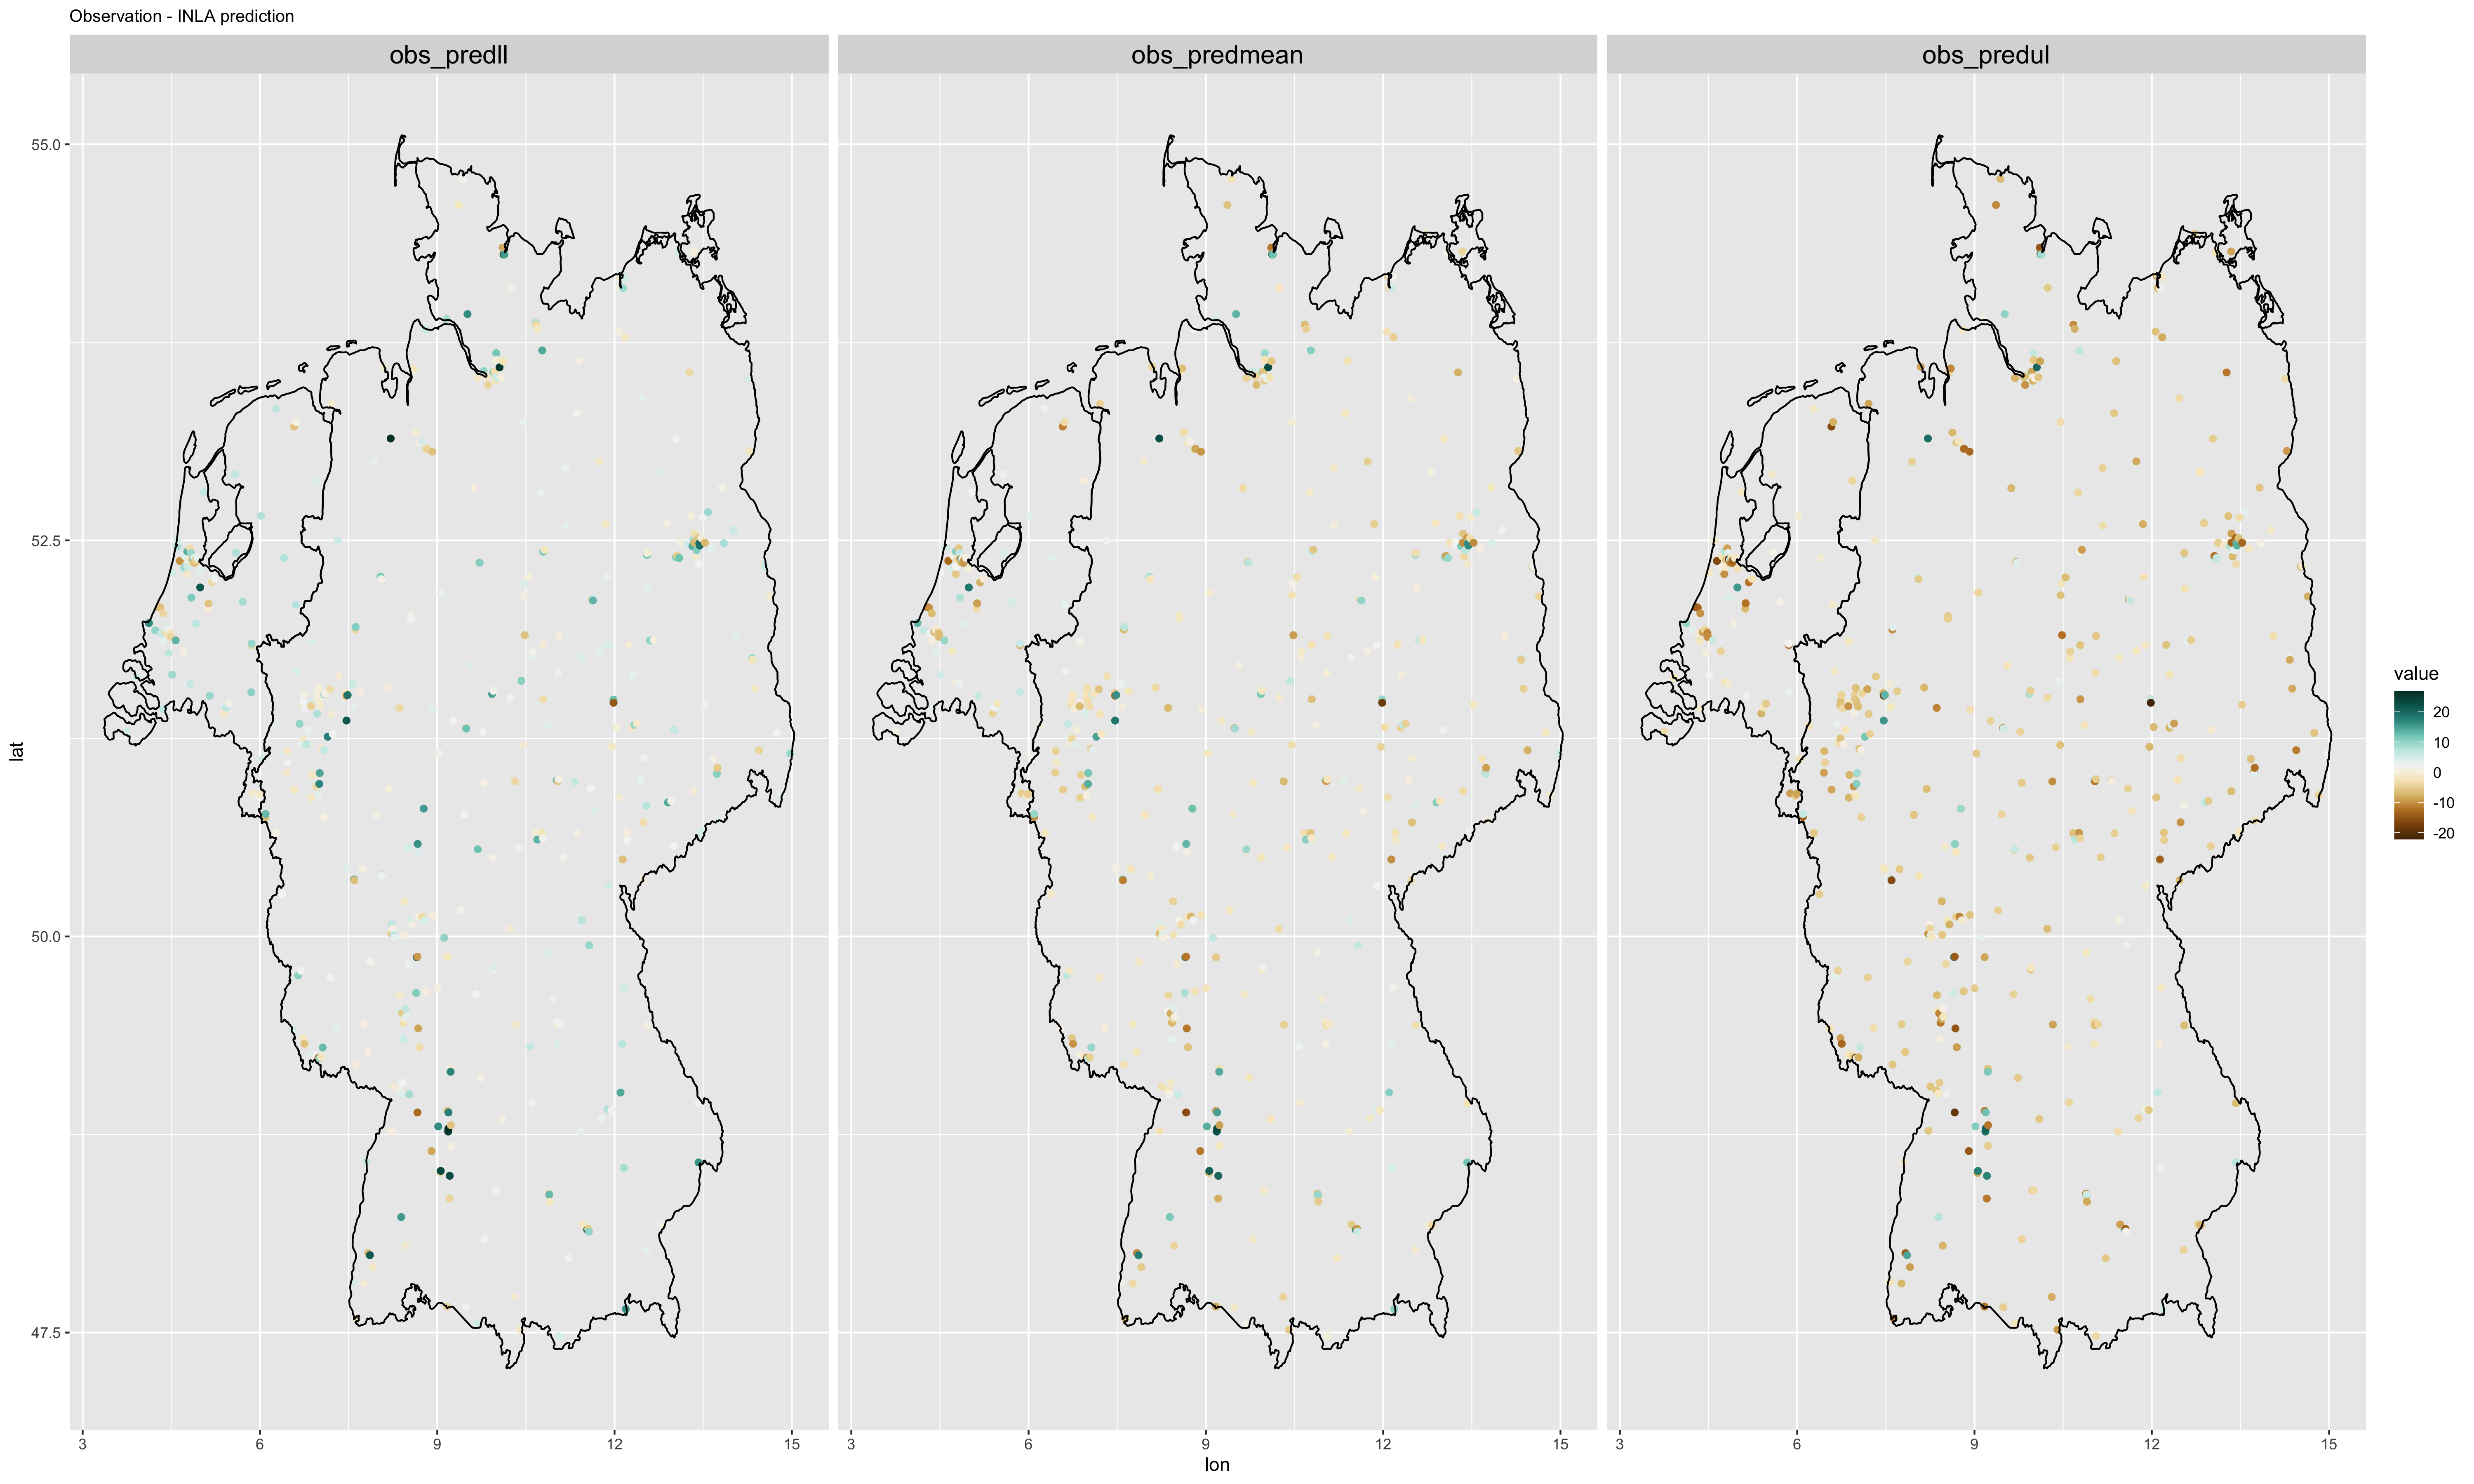
\includegraphics[scale = 0.05]{fig/dif_obs_INLA_11var.png}
\caption{Differences between INLA predicted NO2 at mean, high and low quantiles and the observed NO2. }
\label{difINLA}
\end{figure}

\section{Discussion}
In this study, we compared geostatistical methods with ML methods in spatial NO2 prediction. The comparison consists of the predicted mean, prediction intervals, and model interpretation. The models are evaluated with different CV strategies. We propose the same model evaluation strategies to be incorporated in all the model comparison studies. 

To better predict at boundaries, we experienced with different and large-enough mesh, but this did not improve the performance.
The INLA model without modeling the spatial random effect obtained lower DIC (Information Criterion) 3286.66 vs. 3251.97 (with spatial effects) and WAIC (Watanabe-Akaike information criterion) 3291.75 vs 3253.93 (with spatial effects).  

Different from non-parametric models such as ensemble trees, a parametric model such as the INLA model developed in our study requires feature selection and the assumption of the distribution of the response. Several studies used the whole dataset for variable selection and then use selected variables for CV \citep{lu2020land,larkin2017global}. This may however lead to information leak as the validation data is also used in CV. To avoid this problem, one can include the variable selection process in each CV (i.e. use the same training data for variable selection and test). However, variable selection in each run added in additional error and uncertainty, therefore, a determined set of covariates may be preferred. We obtain fixed set of selected variables while reduce information leakage to a negligible level by choosing only the variables that are selected 90\% -100\% times of all the bootstraps of Lasso.


Deviation from assumed distribution is a common cause of narrow prediction intervals but in our case, assuming a Gamma distribution does not improve model prediction.     

If the prediction interval can be calculated, we can also visualise the uncertainty with the length of a certain quantile of prediction intervals \citep{shaddick2015spatio}.   

Different from Kriging, INLA is a deterministic model and not a statistical method of optimization (e.g. as the maximum likelihood method). As all the estimations are approximations, it is advantageous when use a big number of observations and especially for spatio-temporal models. These are important for extending the model to larger scales (e.g. global-scale) and in space-time. 

Model performance differ between the three road and population situations. the "far" situation obtained the best modelling accuracy while the "tr-hp" the worst. This is likely due to the fact that the urban NO2 process is more complex due to urban forms and traffic conditions. This may also indicates that more detailed traffic counts and meteorological data are needed for modelling the NO2 emission sources.  

\newpage
\bibliographystyle{abbrvnat}

\bibliography{references}
\end{document}

Other: the newest boosting technique, Catboost, gives the best cross validation results, with same learning rate as xgboost and number of iterations. But it's not convenient for now to ensemble it as it is not yet in h2o. 

                    Catboost
RMSE          7.0 
RRMSE         0.3 
IQR           6.4 
rIQR          0.3 
MAE           5.0 
rMAE          0.2 
rsq           0.70 
explained\_var 0.70

with spatial cv
                    INLA 
                    
RMSE          10.0900074
RRMSE          0.3023047
IQR           11.6697717
rIQR           0.3894527
MAE            7.4846970
rMAE           0.2242679
rsq            0.3630397
explained\_var  0.4319317
 
 Lasso
RMSE	10.0900074			
RRMSE	0.3023047			
IQR	11.6697717			
rIQR	0.3894527			
MAE	7.4846970			
rMAE	0.2242679			
rsq	0.3630397			
explained\_var	0.4319317	

RF
RMSE	9.6393525			
RRMSE	0.2888581			
IQR	11.6795936			
rIQR	0.3899266			
MAE	7.2699949			
rMAE	0.2178434			
rsq	0.4176984			
explained\_var	0.4752084			
covprob90	0.9063574	

XGB 
RMSE	9.6618743			
RRMSE	0.2895155			
IQR	10.1181299			
rIQR	0.3379141			
MAE	7.0342845			
rMAE	0.2107836			
rsq	0.4140045			
explained\_var	0.4960338

Stacked INLA
RMSE           8.48140767
RRMSE          0.25475534
IQR           10.50499614
rIQR           0.35099809
MAE            6.53715007
rMAE           0.19644237
rsq            0.54917218
explained\_var  0.55811686
cor            0.75390795
covprob95      0.21804124
covprob90      0.17989691
covprob50      0.08092784


If I choose clustered points with high prob (big city?), the result is similar to random sampling, and better accuracy. 

 

If I choose scattered points with high prob (does it mean more rural points?), there is very little randomness. result is also worse. --> the reason for scattered points with high prob. is because they contain more info?
there are a lot more clustered points (as the hist. peak at small prob). so the scattered points will be selected first, that is the reason there is little randomness. 

 
\subsection{Variable importance}
   \begin{table}[!htbp] \centering 
    \caption{Variable importance ranked by XGBoost and Random Forest. The ranking is based on variable importance averaged over 20 times bootstrapping.} 
    \label{vimp} 
  \begin{tabular}{@{\extracolsep{5pt}} ccc} 
  \\[-1.8ex]\hline 
  \hline \\[-1.8ex] 
  rank & XGBoost & Random Rorest \\ 
  \hline \\[-1.8ex] 
  1 & population\_3000 & population\_3000 \\ 
  2 & road\_class\_3\_3000 & road\_class\_2\_100 \\ 
  3 & population\_1000 & road\_class\_3\_3000 \\ 
  4 & nightlight\_450 & population\_1000 \\ 
  5 & road\_class\_2\_100 & nightlight\_450 \\ 
  6 & road\_class\_3\_300 & nightlight\_3150 \\ 
  7 & road\_class\_1\_5000 & population\_5000 \\ 
  8 & nightlight\_3150 & road\_class\_3\_300 \\ 
  9 & road\_class\_3\_100 & nightlight\_900 \\ 
  10 & population\_5000 & road\_class\_3\_5000 \\ 
  11 & trop\_mean\_filt & road\_class\_2\_300 \\ 
  12 & radiation & road\_class\_3\_100 \\ 
  13 & nightlight\_900 & nightlight\_4950 \\ 
  14 & road\_class\_3\_5000 & trop\_mean\_filt \\ 
  15 & road\_class\_1\_100 & road\_class\_1\_5000 \\ 
  16 & nightlight\_4950 & industry\_5000 \\ 
  17 & temperature\_2m\_2 & road\_class\_1\_3000 \\ 
  18 & road\_class\_1\_3000 & temperature\_2m\_2 \\ 
  19 & elevation & road\_class\_2\_500 \\ 
  20 & industry\_5000 & elevation \\ 
 
  \hline \\[-1.8ex] 
  \end{tabular} 
  \end{table} 
  
  
  \begin{table}[!htbp] \centering 
  \caption{} 
  \label{} 
\begin{tabular}{@{\extracolsep{5pt}} ccccc} 
\\[-1.8ex]\hline 
\hline \\[-1.8ex] 
 & LA & RF & XGB & RFLA \\ 
\hline \\[-1.8ex] 
RMSE & $7.54$ & $7.40$ & $7.10$ & $7.24$ \\ 
RRMSE & $0.32$ & $0.32$ & $0.30$ & $0.31$ \\ 
IQR & $8.42$ & $7.22$ & $6.27$ & $7.26$ \\ 
rIQR & $0.39$ & $0.34$ & $0.29$ & $0.34$ \\ 
MAE & $5.67$ & $5.41$ & $4.98$ & $5.26$ \\ 
rMAE & $0.24$ & $0.23$ & $0.21$ & $0.23$ \\ 
rsq & $0.66$ & $0.67$ & $0.70$ & $0.68$ \\ 
explained\_var & $0.66$ & $0.67$ & $0.70$ & $0.68$ \\ 
\hline \\[-1.8ex] 
\end{tabular} 
\end{table} 

\begin{table}[!htbp] \centering 
  \caption{Cross-validation results of 20 times boot-strapping.} 
  \label{cv} 
\begin{tabular}{@{\extracolsep{5pt}} ccccccc} 
\\[-1.8ex]\hline 
\hline \\[-1.8ex] 
   &LA & RF& XGB & stacked & INLA& stacked INLA  \\ 
\hline \\[-1.8ex] 	
 
RMSE & $7.8$ & $7.5$ & $7.4$ & 7.2 & 7.5&7.1\\
%RRMSE & $0.3$ & $0.3$ & $0.3$&  &0.3\\
IQR & $8.5$ & $7.5$ & $6.9$  &  &7.2\\ % for non-gaussian error this makes little sense
%rIQR & $0.4$ & $0.3$ & $0.3$ & &0.3\\
MAE & $5.9$ & $5.5$ & $5.3$  & 5.2 & 5.5&5.3\\
%rMAE & $0.2$ & $0.2$ & $0.2$ &  &0.2\\
R$^2$ & $0.63$ & $0.66$ & $0.67$&  0.68 &0.66 &0.69\\
%explained\_var & $0.63$ & $0.66$ & $0.67$ &&  0.66 &0.69 \\ 
\hline \\[-1.8ex] 
\end{tabular} 
\end{table} 


%Feb 9, 2021 1:55 PM j.cavieres.g:  If you are talking about the comparison between models (ML, spatial linear models, hierarchical models, etc) based on the distribution of the observed data, I have never seen this. What is my opinion? I think that ML models are more interested in the prediction than in the inference. If they generalize well the prediction of a particular phenomenon then that model is 'good'. In our case it is very interesting to see that the machine learning model using a Gamma distribution has poor statistical performance compared with INLA, but probably that model can predict better. For the above is necessary to do an analysis where we can evaluate if that model is overfitting or not. 